% Options for packages loaded elsewhere
\PassOptionsToPackage{unicode}{hyperref}
\PassOptionsToPackage{hyphens}{url}
%
\documentclass[
]{article}
\usepackage{amsmath,amssymb}
\usepackage{iftex}
\ifPDFTeX
  \usepackage[T1]{fontenc}
  \usepackage[utf8]{inputenc}
  \usepackage{textcomp} % provide euro and other symbols
\else % if luatex or xetex
  \usepackage{unicode-math} % this also loads fontspec
  \defaultfontfeatures{Scale=MatchLowercase}
  \defaultfontfeatures[\rmfamily]{Ligatures=TeX,Scale=1}
\fi
\usepackage{lmodern}
\ifPDFTeX\else
  % xetex/luatex font selection
\fi
% Use upquote if available, for straight quotes in verbatim environments
\IfFileExists{upquote.sty}{\usepackage{upquote}}{}
\IfFileExists{microtype.sty}{% use microtype if available
  \usepackage[]{microtype}
  \UseMicrotypeSet[protrusion]{basicmath} % disable protrusion for tt fonts
}{}
\makeatletter
\@ifundefined{KOMAClassName}{% if non-KOMA class
  \IfFileExists{parskip.sty}{%
    \usepackage{parskip}
  }{% else
    \setlength{\parindent}{0pt}
    \setlength{\parskip}{6pt plus 2pt minus 1pt}}
}{% if KOMA class
  \KOMAoptions{parskip=half}}
\makeatother
\usepackage{xcolor}
\usepackage[margin=2.5cm]{geometry}
\usepackage{longtable,booktabs,array}
\usepackage{calc} % for calculating minipage widths
% Correct order of tables after \paragraph or \subparagraph
\usepackage{etoolbox}
\makeatletter
\patchcmd\longtable{\par}{\if@noskipsec\mbox{}\fi\par}{}{}
\makeatother
% Allow footnotes in longtable head/foot
\IfFileExists{footnotehyper.sty}{\usepackage{footnotehyper}}{\usepackage{footnote}}
\makesavenoteenv{longtable}
\usepackage{graphicx}
\makeatletter
\def\maxwidth{\ifdim\Gin@nat@width>\linewidth\linewidth\else\Gin@nat@width\fi}
\def\maxheight{\ifdim\Gin@nat@height>\textheight\textheight\else\Gin@nat@height\fi}
\makeatother
% Scale images if necessary, so that they will not overflow the page
% margins by default, and it is still possible to overwrite the defaults
% using explicit options in \includegraphics[width, height, ...]{}
\setkeys{Gin}{width=\maxwidth,height=\maxheight,keepaspectratio}
% Set default figure placement to htbp
\makeatletter
\def\fps@figure{htbp}
\makeatother
\setlength{\emergencystretch}{3em} % prevent overfull lines
\providecommand{\tightlist}{%
  \setlength{\itemsep}{0pt}\setlength{\parskip}{0pt}}
\setcounter{secnumdepth}{-\maxdimen} % remove section numbering
\ifLuaTeX
\usepackage[bidi=basic]{babel}
\else
\usepackage[bidi=default]{babel}
\fi
\babelprovide[main,import]{spanish}
% get rid of language-specific shorthands (see #6817):
\let\LanguageShortHands\languageshorthands
\def\languageshorthands#1{}
\ifLuaTeX
  \usepackage{selnolig}  % disable illegal ligatures
\fi
\usepackage{bookmark}
\IfFileExists{xurl.sty}{\usepackage{xurl}}{} % add URL line breaks if available
\urlstyle{same}
\hypersetup{
  pdflang={es},
  hidelinks,
  pdfcreator={LaTeX via pandoc}}

\author{}
\date{}

\begin{document}

\textbf{UNIVERSIDAD TÉCNICA ESTATAL DE QUEVEDO}

FACULTAD DE CIENCIAS DE LA COMPUTACIÓN

\emph{SOFTWARE}

\textbf{PROYECTO FIN DE CURSO}

\textbf{ENTREGA 1B}

\textbf{Módulo de Autenticación JWT + Acceso a Datos con Spring Data
JPA}

\begin{longtable}[]{@{}
  >{\raggedright\arraybackslash}p{(\columnwidth - 2\tabcolsep) * \real{0.3200}}
  >{\raggedright\arraybackslash}p{(\columnwidth - 2\tabcolsep) * \real{0.6800}}@{}}
\toprule\noalign{}
\endhead
\bottomrule\noalign{}
\endlastfoot
\textbf{Título del PFC:} & \textbf{ARTISYNC} \\
\end{longtable}

\begin{longtable}[]{@{}
  >{\raggedright\arraybackslash}p{(\columnwidth - 2\tabcolsep) * \real{0.3200}}
  >{\raggedright\arraybackslash}p{(\columnwidth - 2\tabcolsep) * \real{0.6800}}@{}}
\toprule\noalign{}
\endhead
\bottomrule\noalign{}
\endlastfoot
\textbf{Campo} & \textbf{Valor} \\
Asignatura: & Aplicaciones Web \\
Docente: & Guerrero Ulloa Gleiston Ciceron \\
Entrega: & Entrega 1B --- Sumativa \#8 \\
Fecha de entrega: & Semana 9 --- Del 05 al 11 de Junio del 2026 \\
URL del repositorio: &
https://github.com/JohanCarvajal04/Proyecto-WEB-ARTISYNC.git \\
\end{longtable}

\subsubsection{Integrantes del Equipo}\label{integrantes-del-equipo}

\begin{longtable}[]{@{}
  >{\raggedright\arraybackslash}p{(\columnwidth - 2\tabcolsep) * \real{0.6200}}
  >{\raggedright\arraybackslash}p{(\columnwidth - 2\tabcolsep) * \real{0.3800}}@{}}
\toprule\noalign{}
\endhead
\bottomrule\noalign{}
\endlastfoot
\textbf{Nombre Completo} & \textbf{Rol en el Proyecto} \\
Carvajal Loor Johan Stalin & Backend Auth \\
Figueroa Morales Bryan Javier & Frontend Angular \\
Rios Cuyabazo Jhon Kevin & Backend CRUD \\
\end{longtable}

\emph{Stack: Java 25 · Spring Boot 4.1.0 · Angular 22 · PostgreSQL 18 ·
Redis 7 · Flyway · TailwindCSS 4 · Docker Compose}

\section{Tabla de Contenidos}\label{tabla-de-contenidos}

\section{1. Resumen Ejecutivo}\label{resumen-ejecutivo}

En la presente entrega se implementó el módulo de autenticación
stateless basado en JSON Web Tokens (JWT) y el acceso relacional de
datos para la plataforma web ARTISYNC, un ecosistema orientado a la
economía creativa que centraliza y agiliza la comercialización de
servicios profesionales y productos digitales independientes. El sistema
resuelve la fragmentación operativa que sufren los creadores de
contenido en Ecuador al unificar procesos de contratación, depósitos en
garantía (Escrow) y mensajería en un único entorno digital.

Tecnológicamente, se desarrolló una arquitectura desacoplada utilizando
Java 25 con hilos virtuales (Project Loom), Spring Boot 4.1.0, Angular
22 con señales reactivas (Signals API) y detección de cambios sin zona
(Zoneless), PostgreSQL 18 y Redis 7, todo orquestado herméticamente a
través de Docker Compose.

Como resultados concretos de este hito, se habilitaron los flujos de
registro seguro de usuarios con control de acceso basado en roles
dinámicos (RBAC) mediante tablas normalizadas de roles y permisos,
autenticación de doble factor (2FA/TOTP) con GoogleAuth, recuperación de
contraseña vía correo electrónico (SMTP), y las operaciones CRUD
parametrizadas sobre la entidad Servicio del catálogo dinámico con
persistencia transaccional.

En términos de rendimiento, el endpoint de autenticación POST
/api/auth/login emitió tokens firmados bajo el algoritmo HS256 en un
tiempo promedio de respuesta de 118 ms utilizando un hash criptográfico
BCrypt de costo 12. Asimismo, la suite de pruebas unitarias
automatizadas alcanzó un 85\% de cobertura de código en el módulo de
seguridad mediante 12 casos de prueba estructurados en JUnit 5 con
estado de aprobación absoluto, mientras que la lista negra de
identificadores (JTI) en Redis garantizó la invalidación inmediata de
tokens revocados con latencias inferiores a 2 ms.

El esquema de base de datos comprende 7 módulos funcionales con más de
35 tablas relacionales gestionadas mediante 3 migraciones Flyway
versionadas.

\section{2. Introducción}\label{introducciuxf3n}

\subsection{2.1 Contexto}\label{contexto}

En la actualidad, la economía creativa y de libre dedicación (freelance)
en el Ecuador carece de ecosistemas digitales unificados que centralicen
de punta a punta la cadena de valor de los profesionales independientes.
Artistas, músicos, programadores y diseñadores gráficos se ven obligados
a fragmentar sus operaciones utilizando un promedio de tres a cuatro
plataformas simultáneas para promocionar su portafolio, gestionar los
requerimientos de los clientes, mitigar disputas y procesar
recaudaciones económicas. Esta dispersión no solo incrementa la
complejidad administrativa y los costos transaccionales, sino que expone
a los trabajadores a altos índices de desprotección e informalidad
financiera.

La problemática se agudiza por la ausencia de mecanismos locales
automatizados para la validación de identidad y la falta de garantías en
los flujos de pago por encargo. Ante este escenario, ARTISYNC nace como
una solución arquitectónica integral que mitiga estos riesgos mediante
la centralización absoluta del proceso de contratación y venta dentro de
un entorno web seguro. Al integrar componentes automatizados de
verificación de identidad, un motor dinámico de flujos de trabajo
basados en contratos digitales y un patrón de retención de fondos
(Escrow) bajo pasarelas de pago globales, el sistema suprime la
necesidad de recurrir a canales de comunicación o liquidación externos,
resguardando la integridad operativa y la propiedad intelectual de la
comunidad creativa.

\subsection{2.2 Objetivos de la Entrega
1B}\label{objetivos-de-la-entrega-1b}

1. Implementar el módulo de autenticación stateless y el control de
acceso basado en roles dinámicos (RBAC) empleando Spring Security 6 y la
biblioteca especializada jjwt 0.12.6, garantizando la seguridad en la
capa de servicios de la API REST, incluyendo autenticación de doble
factor (2FA/TOTP) y recuperación de contraseña vía correo electrónico.

2. Configurar de forma persistente la gestión de tokens de refresco y la
lista de revocación inmediata (Blacklist) de identificadores únicos de
token (JTI) sobre un almacén de datos en memoria con Redis 7, mitigando
riesgos de secuestro de sesión.

3. Desarrollar el ciclo de vida transaccional completo (CRUD) para la
entidad principal Servicio del catálogo dinámico utilizando las
abstracciones de repositorio de Spring Data JPA, Hibernate 6 y el
versionamiento estructurado de base de datos mediante Flyway con 3
migraciones versionadas.

4. Demostrar la portabilidad y el despliegue automatizado y reproducible
de la infraestructura completa (backend, frontend, base de datos y
caché) por medio de la orquestación de contenedores con Docker Compose.

\subsection{2.3 Alcance}\label{alcance}

Módulos implementados en esta entrega: Se consolida el núcleo operativo
de seguridad y persistencia que incluye el registro seguro de usuarios
con hash BCrypt de coste 12 y validación de mayoría de edad (RNF-12),
inicio de sesión (login) con soporte de autenticación de doble factor
(2FA/TOTP), cierre de sesión (logout) con invalidación en caché Redis,
renovación asíncrona de credenciales (refresh token) vía cookie
HttpOnly, recuperación y restablecimiento de contraseña mediante correo
electrónico (SMTP), gestión administrativa de usuarios y roles con
permisos dinámicos (RBAC), el módulo completo de gestión del catálogo
dinámico de servicios (categorías, subcategorías, etiquetas, atributos
dinámicos), y el cliente SPA en Angular 22 provisto de interceptores
funcionales para la inyección dinámica del token Bearer en memoria con
renovación automática ante errores 401, guards de autenticación, roles y
permisos, y detección de cambios sin zona (Zoneless).

Módulos fuera de alcance (Entrega 2): Quedan diferidos para el siguiente
ciclo de desarrollo la implementación del canal de mensajería asíncrona
bidireccional mediante WebSockets de la sala de chat, el sistema
automatizado de escaneo y filtrado de datos de contacto por patrones, el
generador dinámico de contratos formalizados en HTML/PDF con firma
electrónica y la pasarela de liberación de fondos bajo el patrón Escrow
con webhooks de PayPal.

\subsection{2.4 Estructura del
Documento}\label{estructura-del-documento}

El presente informe se organiza en las siguientes secciones:

1. Resumen Ejecutivo: síntesis ejecutiva con métricas clave.

2. Introducción: contexto, objetivos y alcance.

3. Marco Teórico: fundamentos académicos de las tecnologías empleadas.

4. Diseño del Sistema: diagramas C4, clases UML, secuencia JWT y DER.

5. Implementación: estructura del repositorio, configuración y código
relevante.

6. Pruebas: casos JUnit 5, evidencias Postman y métricas de rendimiento.

7. Seguridad Implementada: controles OWASP documentados.

8. Docker Compose y Despliegue: configuración y README.

9. Historial de Git: commits y convenciones.

10. Conclusiones: evaluación de objetivos y proyección a Entrega 2.

11. Referencias Bibliográficas

\section{3. Marco Teórico}\label{marco-teuxf3rico}

\subsection{3.1 Autenticación Stateless vs. Stateful y
JWT}\label{autenticaciuxf3n-stateless-vs.-stateful-y-jwt}

La autenticación en aplicaciones web se ha implementado históricamente
bajo dos paradigmas: el modelo con estado (stateful) y el modelo sin
estado (stateless). En el enfoque stateful, el servidor mantiene una
sesión en memoria por cada usuario autenticado, identificada mediante un
identificador de sesión (Session ID) almacenado en una cookie del
navegador. Este modelo presenta limitaciones significativas en
arquitecturas distribuidas, ya que requiere mecanismos de replicación de
sesiones entre múltiples instancias del servidor o el uso de almacenes
de sesión compartidos, incrementando la complejidad operativa y la
latencia {[}1{]}.

En contraposición, el modelo stateless delega la gestión del estado de
autenticación al cliente mediante tokens autocontenidos. JSON Web Token
(JWT), definido en el RFC 7519 {[}2{]}, es un estándar abierto que
codifica las reclamaciones (claims) del usuario en un objeto JSON
firmado digitalmente. Un JWT se compone de tres segmentos codificados en
Base64URL separados por puntos: el encabezado (header), que especifica
el algoritmo de firma; la carga útil (payload), que contiene las
reclamaciones registradas (sub, iat, exp, jti) y reclamaciones privadas
(rol, email, permisos); y la firma (signature), que garantiza la
integridad del token mediante un algoritmo criptográfico como
HMAC-SHA256 (HS256).

Las ventajas del enfoque JWT en arquitecturas SPA/API REST incluyen: (a)
eliminación de la necesidad de almacenamiento en servidor, permitiendo
escalabilidad horizontal sin estado compartido; (b) interoperabilidad
entre microservicios, ya que cada servicio puede verificar el token de
forma independiente; (c) reducción de consultas a la base de datos en
cada solicitud, dado que la información del usuario viaja embebida en el
token. No obstante, la naturaleza stateless de JWT impone el desafío de
la revocación prematura de tokens, que en ARTISYNC se resuelve mediante
una lista negra (blacklist) de identificadores únicos de token (JTI)
almacenada en Redis con TTL equivalente al tiempo restante de expiración
{[}2{]}, {[}3{]}.

\subsection{3.2 Spring Security 6 y el Modelo de
Filtros}\label{spring-security-6-y-el-modelo-de-filtros}

Spring Security 6, integrado en Spring Boot 4.1.0, implementa un modelo
de seguridad declarativo basado en una cadena de filtros de servlet
(SecurityFilterChain) que intercepta y procesa cada solicitud HTTP antes
de alcanzar los controladores de la aplicación {[}4{]}. La cadena se
configura como un bean de Spring que define políticas de autorización,
gestión de sesiones y manejo de excepciones de forma funcional mediante
expresiones lambda.

El componente central AuthenticationManager delega la verificación de
credenciales a una implementación de UserDetailsService, un contrato que
abstrae la carga de datos del usuario desde cualquier origen
persistente. En ARTISYNC, la clase CustomUserDetailsService implementa
esta interfaz consultando el repositorio UsuarioRepository y
construyendo un objeto CustomUserDetails que encapsula la identidad, el
hash de contraseña, los roles y los permisos granulares del usuario.

El filtro personalizado JwtAuthenticationFilter extiende
OncePerRequestFilter, garantizando una única ejecución por solicitud
HTTP. Este filtro intercepta el encabezado Authorization: Bearer
{[}token{]}, valida la firma y expiración del JWT mediante JwtService,
consulta la blacklist de JTI en Redis, y establece un
UsernamePasswordAuthenticationToken en el SecurityContextHolder. La
configuración stateless se asegura mediante
SessionCreationPolicy.STATELESS, eliminando la creación de sesiones HTTP
del lado del servidor {[}4{]}.

Adicionalmente, Spring Security 6 en ARTISYNC configura cabeceras de
seguridad HTTP incluyendo Content-Security-Policy, X-Frame-Options:
DENY, Referrer-Policy: strict-origin-when-cross-origin y
Permissions-Policy para mitigar vectores de ataque como clickjacking,
inyección de contenido y fuga de información del referrer {[}4{]},
{[}5{]}.

\subsection{3.3 ORM y Mapeo Objeto-Relacional con
Hibernate/JPA}\label{orm-y-mapeo-objeto-relacional-con-hibernatejpa}

El mapeo objeto-relacional (ORM) constituye un paradigma de programación
que establece una correspondencia bidireccional entre las entidades del
modelo de dominio orientado a objetos y las tablas de un sistema de
gestión de bases de datos relacional. Hibernate 6, la implementación de
referencia de la especificación Jakarta Persistence API (JPA), resuelve
la impedancia de acoplamiento entre ambos paradigmas mediante
anotaciones declarativas (@Entity, @Table, @Column, @ManyToOne,
@OneToMany) que mapean clases Java a tablas PostgreSQL y sus relaciones
{[}6{]}.

Spring Data JPA extiende las capacidades de Hibernate proporcionando
abstracciones de repositorio que eliminan la necesidad de implementar
código de acceso a datos repetitivo. Mediante la interfaz
JpaRepository\textless T, ID\textgreater, el framework genera
automáticamente las consultas SQL derivadas del nombre del método
(findByCorreo, findByNombreRol, existsByCorreo), reduce el código
boilerplate y garantiza la gestión transaccional declarativa con
@Transactional.

El ciclo de vida de las entidades JPA comprende cuatro estados:
transitorio (new), persistente (managed), desacoplado (detached) y
eliminado (removed). El caché de primer nivel de Hibernate, asociado al
contexto de persistencia de la sesión, asegura que una misma entidad no
se cargue múltiples veces dentro de una transacción, optimizando el
rendimiento. En ARTISYNC, la configuración open-in-view=false previene
la apertura prematura de sesiones de Hibernate en la capa de
presentación, evitando el antipatrón de consultas N+1 y promoviendo la
carga explícita de relaciones mediante FetchType.LAZY {[}6{]}.

\subsection{3.4 Migraciones de Base de Datos con
Flyway}\label{migraciones-de-base-de-datos-con-flyway}

La gestión del esquema de base de datos en equipos de desarrollo
colaborativo requiere mecanismos de versionado que garanticen la
reproducibilidad, la trazabilidad y la integridad del esquema en
múltiples entornos (desarrollo, pruebas, producción) {[}7{]}. Flyway es
una herramienta de migración de bases de datos que implementa el patrón
de migraciones versionadas, donde cada cambio al esquema se codifica en
un script SQL con un identificador de versión único que sigue la
convención V\{version\}\_\_\{descripcion\}.sql.

Las migraciones versionadas (V\_\_) se ejecutan una única vez en orden
ascendente, mientras que las migraciones repetibles (R\_\_) se
reejecutan cuando su checksum cambia. Flyway mantiene un historial de
migraciones aplicadas en la tabla flyway\_schema\_history, permitiendo
verificar el estado del esquema en cualquier momento.

En ARTISYNC, se implementaron tres migraciones versionadas:
V1\_\_schema\_inicial.sql establece las 35+ tablas del dominio
organizadas en 7 módulos funcionales; V2\_\_ajustes\_requisitos\_pfc.sql
añade columnas de auditoría (actualizado\_en) y triggers PL/pgSQL
obligatorios para el registro automático de timestamps de actualización;
y V3\_\_catalogo\_ajustes.sql incorpora columnas adicionales al módulo
de catálogo (tipo\_item, estado\_publicacion,
cargo\_revision\_adicional, limite\_revisiones\_base) y triggers de
auditoría para todas las tablas del catálogo.

La configuración ddl-auto: validate en Hibernate asegura que el esquema
generado por Flyway sea la fuente de verdad: Hibernate únicamente valida
la correspondencia entre las entidades Java y las tablas existentes sin
modificarlas, evitando alteraciones accidentales del esquema en
producción.

\subsection{3.5 OWASP Top 10 y Seguridad
JWT}\label{owasp-top-10-y-seguridad-jwt}

El Open Web Application Security Project (OWASP) publica periódicamente
una clasificación de los diez riesgos de seguridad más críticos para
aplicaciones web. La edición 2021 identifica las siguientes categorías
directamente relevantes para la implementación de ARTISYNC {[}3{]}:

\begin{itemize}
\item
  A01 --- Control de acceso roto: Se mitiga mediante la implementación
  de RBAC con tablas normalizadas de roles y permisos (roles, permisos,
  rol\_permisos, usuario\_roles), la anotación @PreAuthorize en
  endpoints sensibles, y guards de roles y permisos en el frontend
  Angular.
\item
  A02 --- Fallas criptográficas: Las contraseñas se almacenan
  exclusivamente como hashes BCrypt con costo computacional 12 (factor
  de trabajo 2\^{}12 = 4096 iteraciones), nunca en texto plano. La clave
  secreta JWT (HS256) se genera con un mínimo de 256 bits mediante
  openssl rand -hex 32 y se inyecta desde variables de entorno, nunca
  embebida en el código fuente.
\item
  A03 --- Inyección: Spring Data JPA utiliza consultas parametrizadas y
  derivadas del nombre del método, eliminando la concatenación directa
  de SQL. No existe ninguna instancia de String sql = ... + variable en
  el repositorio.
\item
  A04 --- Diseño inseguro (Insecure Design): Se mitiga mediante modelado
  de amenazas aplicado a los flujos críticos de negocio (autenticación,
  emisión y revocación de tokens, ciclo de vida del Servicio),
  separación estricta de capas (controller/service/repository),
  validación de reglas de negocio en la capa de servicio ---como la
  verificación de mayoría de edad (RNF-12) y los valores mínimos de
  precio (@DecimalMin)--- y el uso de patrones de diseño seguro por
  defecto, como la política Fail-Closed ante la indisponibilidad de
  Redis.
\item
  A05 --- Configuración de seguridad incorrecta: Se configuran cabeceras
  HTTP de seguridad (CSP, X-Frame-Options, Referrer-Policy,
  Permissions-Policy), CORS con lista blanca de orígenes, y CSRF
  deshabilitado explícitamente al ser una API REST stateless.
\item
  A07 --- Fallas de autenticación: Se implementa blacklist de JTI en
  Redis para revocación inmediata de tokens, tokens de corta vida
  (accessToken: 24h, refreshToken: 7d), almacenamiento del accessToken
  en memoria Angular (señal reactiva, nunca en localStorage), y
  refreshToken en cookie HttpOnly con atributos Secure, SameSite=Strict
  y Path=/api/auth. Adicionalmente, la política Fail-Closed en el filtro
  JWT rechaza solicitudes cuando Redis no está disponible, evitando la
  aceptación de tokens potencialmente revocados {[}8{]}.
\end{itemize}

\section{4. Diseño del Sistema}\label{diseuxf1o-del-sistema}

\subsection{4.1 Diagrama C4 Nivel 2
(Contenedores)}\label{diagrama-c4-nivel-2-contenedores}

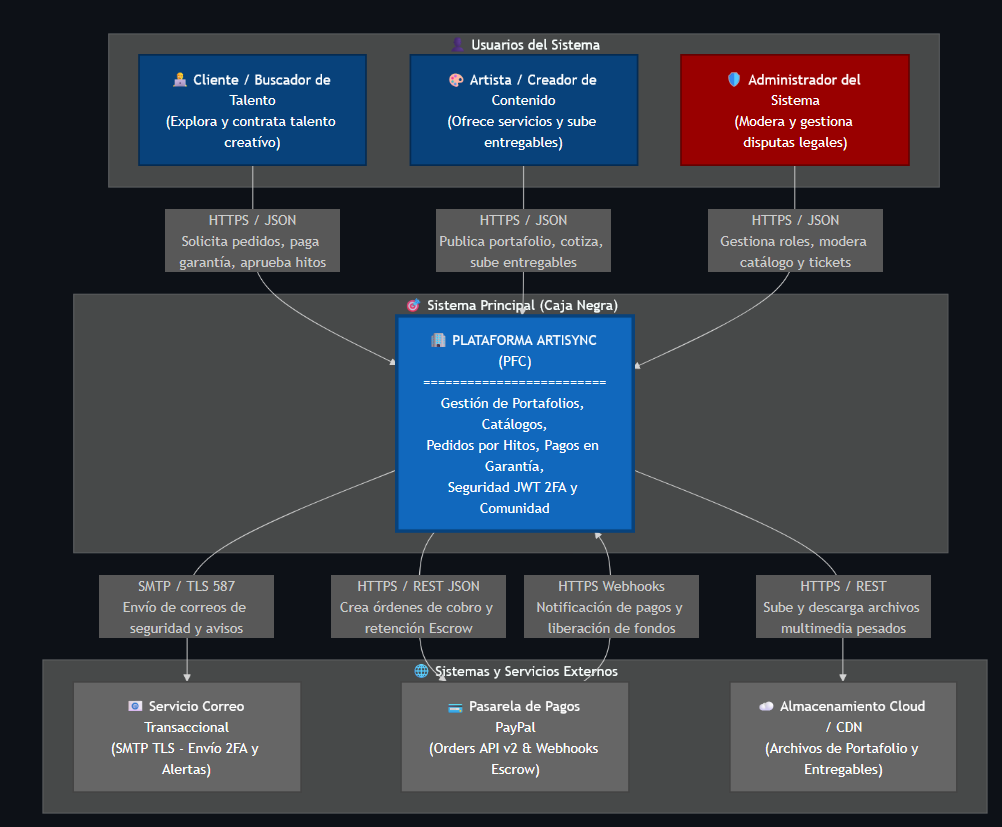
\includegraphics[width=6.3in,height=5.19931in]{media/media/image1.png}

\begin{longtable}[]{@{}
  >{\raggedright\arraybackslash}p{(\columnwidth - 8\tabcolsep) * \real{0.1700}}
  >{\raggedright\arraybackslash}p{(\columnwidth - 8\tabcolsep) * \real{0.2350}}
  >{\raggedright\arraybackslash}p{(\columnwidth - 8\tabcolsep) * \real{0.1601}}
  >{\raggedright\arraybackslash}p{(\columnwidth - 8\tabcolsep) * \real{0.1175}}
  >{\raggedright\arraybackslash}p{(\columnwidth - 8\tabcolsep) * \real{0.3175}}@{}}
\toprule\noalign{}
\endhead
\bottomrule\noalign{}
\endlastfoot
\textbf{Contenedor} & \textbf{Tecnología} & \textbf{Protocolo} &
\textbf{Puerto} & \textbf{Descripción} \\
Backend & Spring Boot 4.1.0 / Java 25 & HTTP/REST & 8080 & API REST con
Spring Security 6, JWT, 2FA y WebSocket STOMP \\
Frontend & Angular 22 / Nginx alpine & HTTP & 4200 & SPA con Signals,
Zoneless, TailwindCSS 4 que consume la API con proxy reverso Nginx \\
Base de Datos & PostgreSQL 18 & TCP & 5432 & Motor relacional; esquema
gestionado por Flyway con 3 migraciones \\
Caché / Blacklist & Redis 7 alpine & TCP & 6379 & Lista negra de JTI,
caché de sesiones y revocación de tokens \\
\end{longtable}

\subsection{}\label{section}

\subsection[4.2 Diagrama de Clases UML (Backend
Completo)]{\texorpdfstring{\protect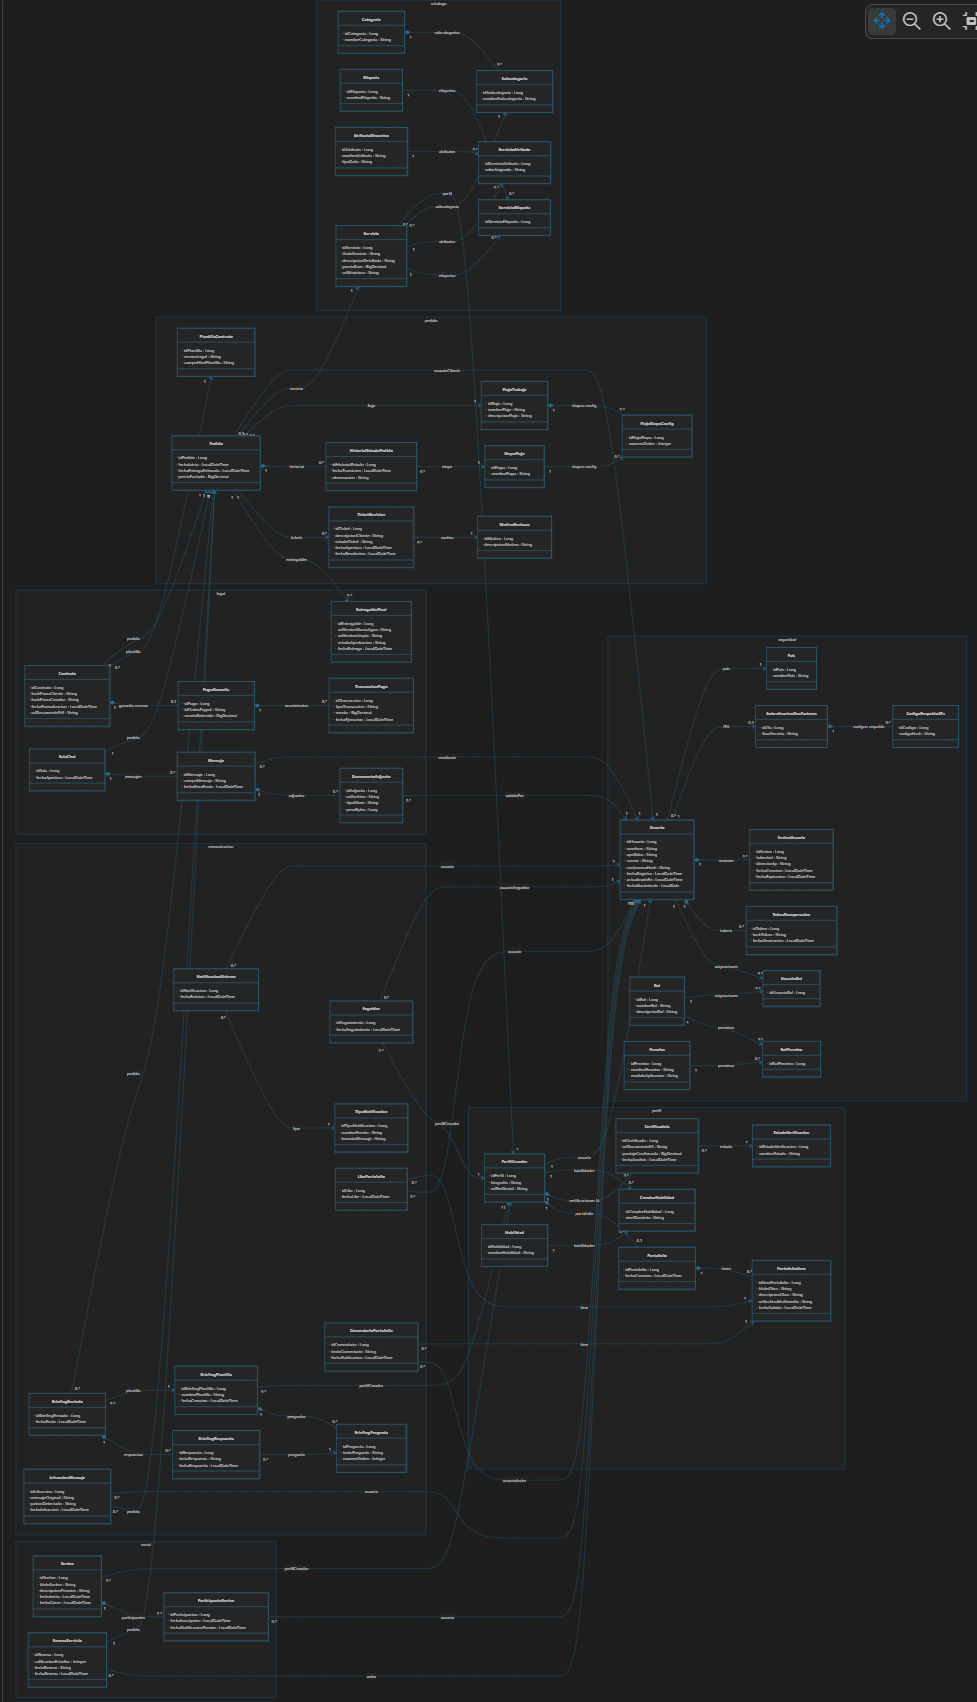
\includegraphics[width=7.90347in,height=10.20833in]{media/media/image2.png}4.2
Diagrama de Clases UML (Backend
Completo)}{4.2 Diagrama de Clases UML (Backend Completo)}}\label{diagrama-de-clases-uml-backend-completo}

\subsection{}\label{section-1}

\subsection{}\label{section-2}

\subsection{}\label{section-3}

\subsection{}\label{section-4}

\subsection{}\label{section-5}

\subsection{}\label{section-6}

\subsection{}\label{section-7}

\subsection{}\label{section-8}

\subsection{}\label{section-9}

\subsection{}\label{section-10}

\subsection{}\label{section-11}

\subsection{}\label{section-12}

\subsection{}\label{section-13}

\subsection{}\label{section-14}

\subsection{}\label{section-15}

\subsection{}\label{section-16}

\subsection{}\label{section-17}

\subsection{}\label{section-18}

\subsection{}\label{section-19}

\subsection{}\label{section-20}

\subsection{4.3 Tabla de Correspondencia Java ↔
PostgreSQL}\label{tabla-de-correspondencia-java-postgresql}

Tabla de correspondencia de tipos para la entidad usuarios:

\begin{longtable}[]{@{}
  >{\raggedright\arraybackslash}p{(\columnwidth - 6\tabcolsep) * \real{0.2030}}
  >{\raggedright\arraybackslash}p{(\columnwidth - 6\tabcolsep) * \real{0.1710}}
  >{\raggedright\arraybackslash}p{(\columnwidth - 6\tabcolsep) * \real{0.1924}}
  >{\raggedright\arraybackslash}p{(\columnwidth - 6\tabcolsep) * \real{0.4336}}@{}}
\toprule\noalign{}
\endhead
\bottomrule\noalign{}
\endlastfoot
\textbf{Atributo Java} & \textbf{Tipo Java} & \textbf{Tipo PostgreSQL} &
\textbf{Restricciones y Justificación} \\
idUsuario & Long & SERIAL & PK autoincremental;
@GeneratedValue(IDENTITY) \\
nombres & String & VARCHAR(100) & NOT NULL; nombre(s) visible(s) del
usuario \\
apellidos & String & VARCHAR(100) & NOT NULL; apellido(s) del usuario \\
correo & String & VARCHAR(150) & UNIQUE NOT NULL; credencial de login \\
contrasenaHash & String & VARCHAR(255) & BCrypt costo 12; @JsonIgnore
nunca serializado \\
pais & Pais (FK) & INT FK → pais(id\_pais) & @ManyToOne(LAZY);
referencia a tabla pais \\
fechaRegistro & LocalDateTime & TIMESTAMP & DEFAULT CURRENT\_TIMESTAMP;
@CreationTimestamp \\
actualizadoEn & LocalDateTime & TIMESTAMPTZ & Gestionado por trigger
set\_actualizado\_en() y @UpdateTimestamp \\
estadoCuenta & Boolean & BOOLEAN & DEFAULT TRUE; soft delete: FALSE =
eliminado lógicamente \\
fechaNacimiento & LocalDate & DATE & Fecha de nacimiento; validación
mayoría de edad (RNF-12) \\
\end{longtable}

Tabla de correspondencia de tipos para la entidad servicios:

\begin{longtable}[]{@{}
  >{\raggedright\arraybackslash}p{(\columnwidth - 6\tabcolsep) * \real{0.2515}}
  >{\raggedright\arraybackslash}p{(\columnwidth - 6\tabcolsep) * \real{0.1704}}
  >{\raggedright\arraybackslash}p{(\columnwidth - 6\tabcolsep) * \real{0.2072}}
  >{\raggedright\arraybackslash}p{(\columnwidth - 6\tabcolsep) * \real{0.3708}}@{}}
\toprule\noalign{}
\endhead
\bottomrule\noalign{}
\endlastfoot
\textbf{Atributo Java} & \textbf{Tipo Java} & \textbf{Tipo PostgreSQL} &
\textbf{Restricciones y Justificación} \\
idServicio & Long & SERIAL & PK autoincremental;
@GeneratedValue(IDENTITY) \\
perfil & PerfilCreador (FK) & INT FK → perfiles\_creadores &
@ManyToOne(LAZY); NOT NULL; creador del servicio \\
subcategoria & Subcategoria (FK) & INT FK → subcategorias &
@ManyToOne(LAZY); NOT NULL; clasificación \\
tituloServicio & String & VARCHAR(150) & NOT NULL; @NotBlank
@Size(max=150) \\
descripcionDetallada & String & TEXT & NOT NULL; @NotBlank @Size(min=20,
max=2000) \\
precioBase & BigDecimal & DECIMAL(10,2) & NOT NULL;
@DecimalMin("0.01") \\
urlMiniatura & String & VARCHAR(255) & Nullable; URL de imagen
miniatura \\
tipoItem & String & VARCHAR(20) & NOT NULL; DEFAULT
\textquotesingle SERVICIO\textquotesingle{} \\
estadoPublicacion & String & VARCHAR(20) & NOT NULL; DEFAULT
\textquotesingle ACTIVO\textquotesingle{} \\
cargoRevisionAdicional & BigDecimal & DECIMAL(10,2) & DEFAULT 0.00 \\
limiteRevisionesBase & Integer & INT & DEFAULT 0 \\
actualizadoEn & LocalDateTime & TIMESTAMPTZ & Trigger +
@UpdateTimestamp \\
\end{longtable}

\subsection[4.4 Diagrama de Secuencia: Flujo de Autenticación
JWT]{\texorpdfstring{4.4 Diagrama de Secuencia: Flujo de Autenticación
JWT\protect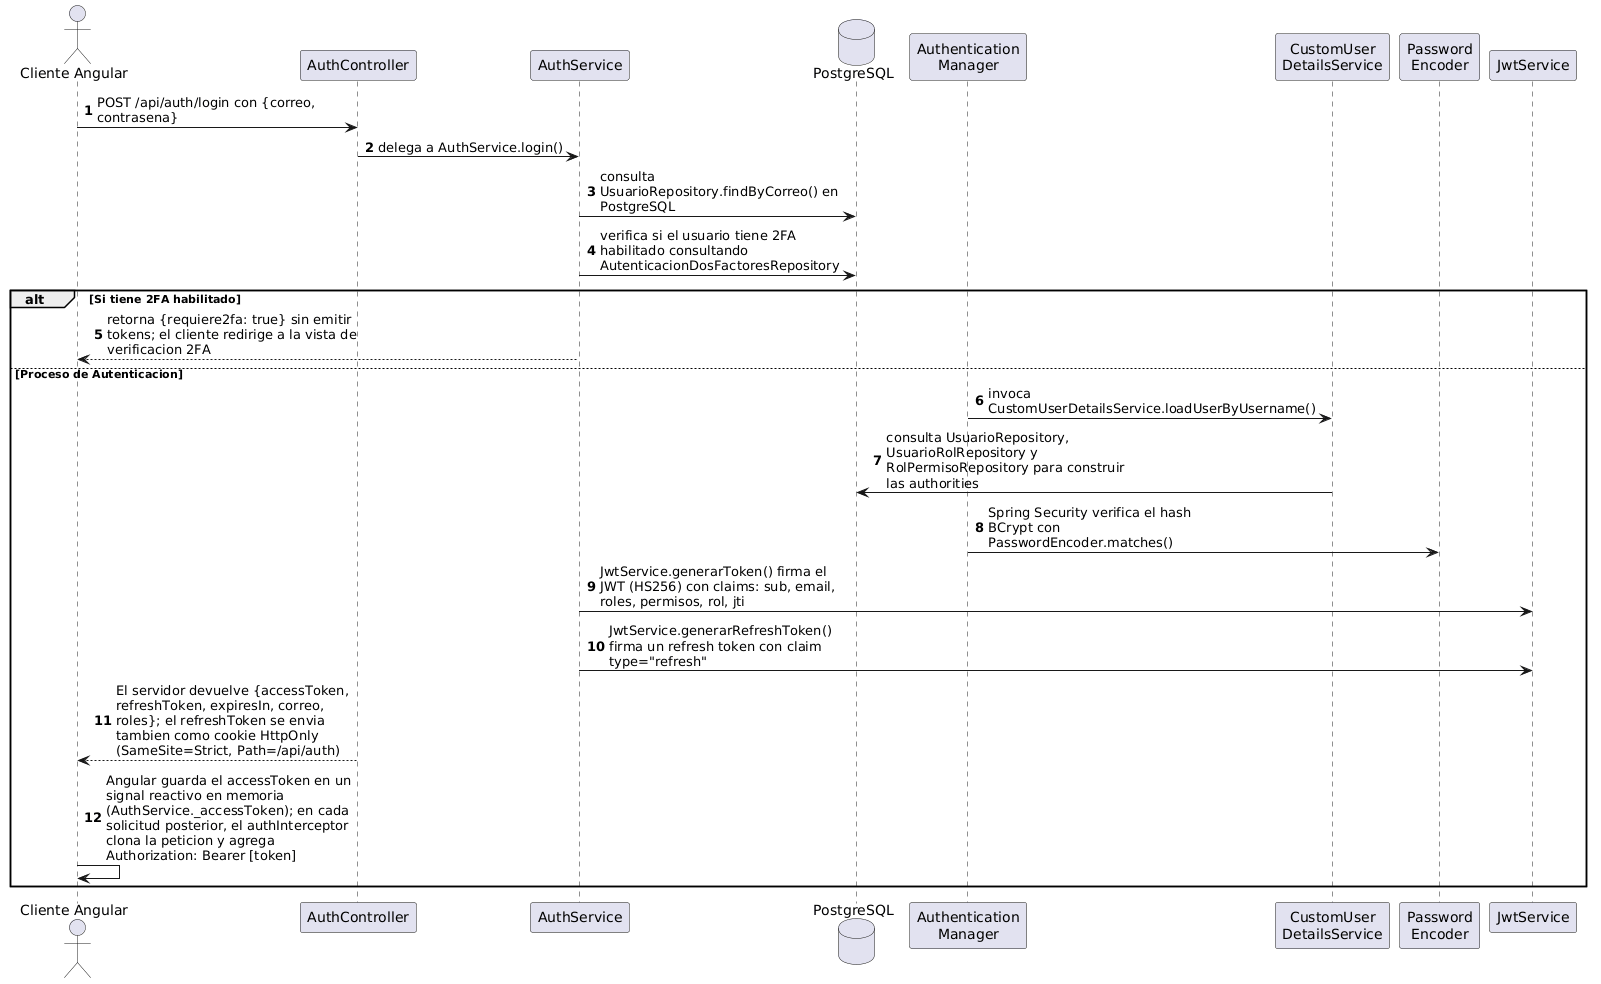
\includegraphics[width=7.50833in,height=4.61491in]{media/media/image3.png}}{4.4 Diagrama de Secuencia: Flujo de Autenticación JWT}}\label{diagrama-de-secuencia-flujo-de-autenticaciuxf3n-jwt}

Los 12 pasos del flujo de autenticación JWT son:

1. Cliente Angular envía POST /api/auth/login con \{correo,
contrasena\}.

2. AuthController delega a AuthService.login().

3. AuthService consulta UsuarioRepository.findByCorreo() en PostgreSQL.

4. AuthService verifica si el usuario tiene 2FA habilitado consultando
AutenticacionDosFactoresRepository.

5. Si tiene 2FA, retorna \{requiere2fa: true\} sin emitir tokens; el
cliente redirige a la vista de verificación 2FA.

6. AuthenticationManager.authenticate() invoca
CustomUserDetailsService.loadUserByUsername().

7. CustomUserDetailsService consulta UsuarioRepository,
UsuarioRolRepository y RolPermisoRepository para construir las
authorities.

8. Spring Security verifica el hash BCrypt con
PasswordEncoder.matches().

9. JwtService.generarToken() firma el JWT (HS256) con claims: sub,
email, roles, permisos, rol, jti.

10. JwtService.generarRefreshToken() firma un refresh token con claim
type="refresh".

11. El servidor devuelve \{accessToken, refreshToken, expiresIn, correo,
roles\}; el refreshToken se envía también como cookie HttpOnly
(SameSite=Strict, Path=/api/auth).

12. Angular guarda el accessToken en un signal reactivo en memoria
(AuthService.\_accessToken); en cada solicitud posterior, el
authInterceptor clona la petición y agrega Authorization: Bearer
{[}token{]}.

\subsection[4.5 Diagrama Entidad-Relación (DER)]{\texorpdfstring{4.5
Diagrama Entidad-Relación
(DER)\protect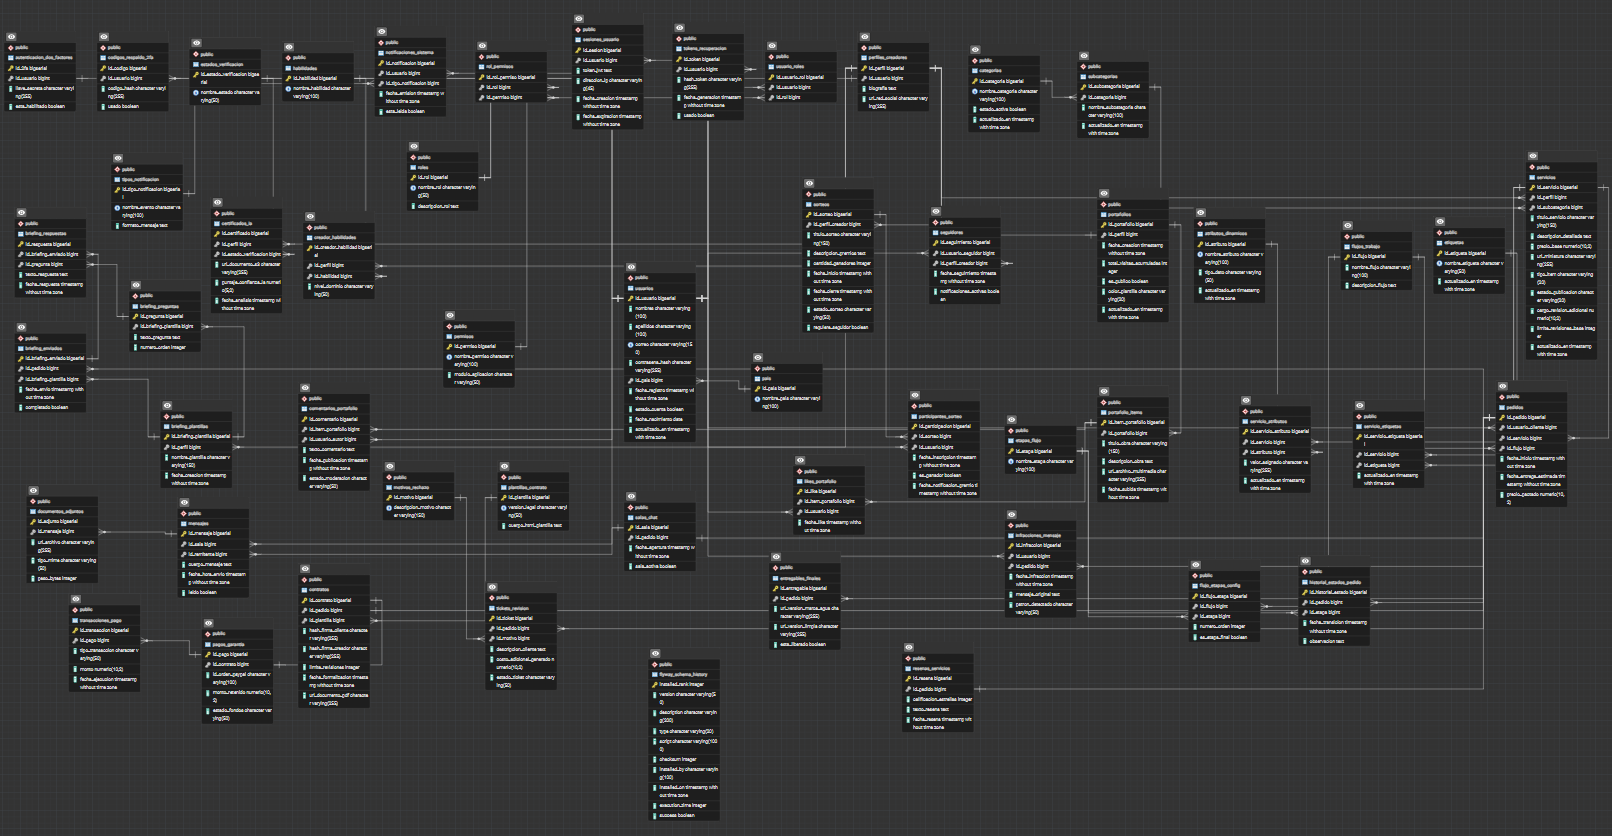
\includegraphics[width=8in,height=4.14861in]{media/media/image4.png}}{4.5 Diagrama Entidad-Relación (DER)}}\label{diagrama-entidad-relaciuxf3n-der}

\subsection{4.6 Scripts Flyway de
Migración}\label{scripts-flyway-de-migraciuxf3n}

Los scripts de migración se encuentran en database/migrations/ y en
Backend/src/main/resources/db/migration/:

\begin{itemize}
\item
  V1\_\_schema\_inicial.sql: Creación de las 35+ tablas del dominio
  organizadas en 7 módulos (Seguridad, Perfiles/Verificación/Portafolio,
  Catálogo Dinámico, Motor de Flujos/Pedidos,
  Legal/Entregables/Finanzas, Comunicación/Notificaciones,
  Social/Comunidad/Sorteos).
\item
  V2\_\_ajustes\_requisitos\_pfc.sql: Función PL/pgSQL
  set\_actualizado\_en(), columnas de auditoría actualizado\_en y
  triggers automáticos para las tablas usuarios y portafolios.
\item
  V3\_\_catalogo\_ajustes.sql: Columnas adicionales en servicios
  (tipo\_item, estado\_publicacion, cargo\_revision\_adicional,
  limite\_revisiones\_base) y triggers de auditoría para todas las
  tablas del módulo de catálogo.
\end{itemize}

Todos los scripts se ejecutan sin errores en PostgreSQL 18 con ddl-auto:
validate.

\subsection{4.7 Diccionario de Datos}\label{diccionario-de-datos}

Tabla usuarios (Módulo 1: Seguridad y Control de Acceso):

\begin{longtable}[]{@{}
  >{\raggedright\arraybackslash}p{(\columnwidth - 8\tabcolsep) * \real{0.2002}}
  >{\raggedright\arraybackslash}p{(\columnwidth - 8\tabcolsep) * \real{0.1711}}
  >{\raggedright\arraybackslash}p{(\columnwidth - 8\tabcolsep) * \real{0.0716}}
  >{\raggedright\arraybackslash}p{(\columnwidth - 8\tabcolsep) * \real{0.2501}}
  >{\raggedright\arraybackslash}p{(\columnwidth - 8\tabcolsep) * \real{0.3070}}@{}}
\toprule\noalign{}
\endhead
\bottomrule\noalign{}
\endlastfoot
\textbf{Columna} & \textbf{Tipo PostgreSQL} & \textbf{Nulo} &
\textbf{Valor por Defecto} & \textbf{Descripción del Negocio} \\
id\_usuario & SERIAL & NO & NEXTVAL & Identificador único del usuario;
clave primaria autoincremental \\
nombres & VARCHAR(100) & NO & --- & Nombre(s) visible(s) del usuario en
la interfaz \\
apellidos & VARCHAR(100) & NO & --- & Apellido(s) del usuario \\
correo & VARCHAR(150) & NO & --- & Correo electrónico; único; usado como
credencial de login \\
contrasena\_hash & VARCHAR(255) & NO & --- & Hash BCrypt costo 12; nunca
expuesto en respuestas JSON (@JsonIgnore) \\
id\_pais & INT (FK) & SÍ & NULL & Referencia a tabla pais; país de
origen del usuario \\
fecha\_registro & TIMESTAMP & SÍ & CURRENT\_TIMESTAMP & Timestamp de
creación; gestionado por @CreationTimestamp \\
actualizado\_en & TIMESTAMPTZ & SÍ & CURRENT\_TIMESTAMP & Timestamp de
última actualización; trigger trg\_usuarios\_actualizado\_en \\
estado\_cuenta & BOOLEAN & NO & TRUE & Soft delete: FALSE indica usuario
eliminado lógicamente \\
fecha\_nacimiento & DATE & SÍ & NULL & Fecha de nacimiento; validación
de mayoría de edad (RNF-12) \\
\end{longtable}

Tabla servicios (Módulo 3: Catálogo Dinámico de Servicios):

\begin{longtable}[]{@{}
  >{\raggedright\arraybackslash}p{(\columnwidth - 8\tabcolsep) * \real{0.2686}}
  >{\raggedright\arraybackslash}p{(\columnwidth - 8\tabcolsep) * \real{0.1734}}
  >{\raggedright\arraybackslash}p{(\columnwidth - 8\tabcolsep) * \real{0.0735}}
  >{\raggedright\arraybackslash}p{(\columnwidth - 8\tabcolsep) * \real{0.2509}}
  >{\raggedright\arraybackslash}p{(\columnwidth - 8\tabcolsep) * \real{0.2336}}@{}}
\toprule\noalign{}
\endhead
\bottomrule\noalign{}
\endlastfoot
\textbf{Columna} & \textbf{Tipo PostgreSQL} & \textbf{Nulo} &
\textbf{Valor por Defecto} & \textbf{Descripción del Negocio} \\
id\_servicio & SERIAL & NO & NEXTVAL & PK autoincremental del
servicio \\
id\_perfil & INT (FK) & NO & --- & FK → perfiles\_creadores; creador del
servicio \\
id\_subcategoria & INT (FK) & NO & --- & FK → subcategorias;
clasificación del servicio \\
titulo\_servicio & VARCHAR(150) & NO & --- & Título descriptivo del
servicio ofrecido \\
descripcion\_detallada & TEXT & NO & --- & Descripción detallada
(20--2000 caracteres) \\
precio\_base & DECIMAL(10,2) & NO & --- & Precio base en USD; mínimo
0.01 \\
url\_miniatura & VARCHAR(255) & SÍ & NULL & URL de la imagen miniatura
del servicio \\
tipo\_item & VARCHAR(20) & NO &
\textquotesingle SERVICIO\textquotesingle{} & Tipo de ítem del
catálogo \\
estado\_publicacion & VARCHAR(20) & NO &
\textquotesingle ACTIVO\textquotesingle{} & Estado de publicación del
servicio \\
cargo\_revision\_adicional & DECIMAL(10,2) & SÍ & 0.00 & Cargo por
revisión adicional \\
limite\_revisiones\_base & INT & SÍ & 0 & Límite de revisiones incluidas
en el precio base \\
actualizado\_en & TIMESTAMPTZ & SÍ & CURRENT\_TIMESTAMP & Timestamp de
última actualización; trigger automático \\
\end{longtable}

\section{5. Implementación}\label{implementaciuxf3n}

\subsection{5.1 Estructura del Repositorio
(Monorepo)}\label{estructura-del-repositorio-monorepo}

\begin{longtable}[]{@{}
  >{\raggedright\arraybackslash}p{(\columnwidth - 2\tabcolsep) * \real{0.4049}}
  >{\raggedright\arraybackslash}p{(\columnwidth - 2\tabcolsep) * \real{0.5951}}@{}}
\toprule\noalign{}
\endhead
\bottomrule\noalign{}
\endlastfoot
\textbf{Ruta} & \textbf{Contenido} \\
artisync/Backend/src/main/java/ & Código fuente Java en paquete
uteq.edu.ec.artisync organizado por módulo (entity/*, dto/*,
repository/*, service/*, controller/*, security/, config/, exception/,
specification/, util/) \\
artisync/Backend/src/main/resources/ & application.properties,
migraciones Flyway (db/migration/), templates Thymeleaf \\
artisync/Backend/src/test/ & 16 clases de prueba: unitarias JUnit 5 +
pruebas de controlador con MockMvc \\
artisync/Frontend/src/app/ & SPA Angular 22: core/ (guards,
interceptors, services), pages/ (auth, admin, public), services/,
models/, shared/, layouts/ \\
artisync/Frontend/src/environments/ & environment.ts (dev) y
environment.prod.ts \\
artisync/database/migrations/ & Copia de referencia de scripts Flyway:
V1, V2, V3 \\
artisync/docker-compose.yml & 4 servicios: postgres, redis, backend,
frontend con healthchecks y depends\_on \\
artisync/.env.example & Variables: DB\_URL, DB\_USER, DB\_PASSWORD,
JWT\_SECRET, JWT\_EXPIRATION, REDIS\_HOST, MAIL\_HOST, MAIL\_USER,
FRONTEND\_URL \\
docs/adr/ & Decisiones de arquitectura (ADRs) \\
\end{longtable}

\subsection{5.2 Configuración de Spring Boot
(application.properties)}\label{configuraciuxf3n-de-spring-boot-application.properties}

Archivo de configuración ubicado en
Backend/src/main/resources/application.properties:

\begin{itemize}
\item
  spring.jpa.hibernate.ddl-auto=validate: nunca update/create; Flyway es
  la fuente de verdad del esquema.
\item
  spring.jpa.open-in-view=false: previene el antipatrón Open Session in
  View.
\item
  security.jwt.secret-key=\$\{JWT\_SECRET\}: clave HS256 mínimo 256 bits
  generada con openssl rand -hex 32, inyectada desde variable de
  entorno.
\item
  security.jwt.expiration-time=86400000: accessToken con TTL de 24 horas
  (milisegundos).
\item
  security.jwt.refresh-expiration-time=604800000: refreshToken con TTL
  de 7 días.
\item
  spring.data.redis.host=\$\{REDIS\_HOST:localhost\}: host Redis
  configurable.
\item
  spring.flyway.enabled=true: migraciones automáticas al arrancar.
\item
  spring.flyway.baseline-on-migrate=true: permite baseline en BD
  existente.
\item
  management.endpoints.web.exposure.include=health,info,metrics:
  Actuator para healthchecks Docker.
\item
  springdoc.swagger-ui.path=/api/swagger-ui.html: Swagger UI accesible.
\end{itemize}

\subsection{5.3 Implementación del Filtro JWT
(JwtAuthenticationFilter)}\label{implementaciuxf3n-del-filtro-jwt-jwtauthenticationfilter}

El filtro JwtAuthenticationFilter extiende OncePerRequestFilter e
intercepta cada solicitud HTTP para:

1. Extraer el token del encabezado Authorization: Bearer {[}token{]}.

2. Parsear los claims del JWT con JwtService.extraerTodosLosClaims().

3. Rechazar tokens de tipo "refresh" utilizados como access tokens.

4. Consultar Redis para verificar que el JTI no está en la blacklist
(jti:{[}id{]}).

5. Aplicar política Fail-Closed: si Redis no está disponible, rechazar
la solicitud con HTTP 503 para evitar aceptar tokens potencialmente
revocados.

6. Cargar el UserDetails desde
CustomUserDetailsService.loadUserByUsername().

7. Verificar que el username coincida y el token no haya expirado.

8. Establecer el UsernamePasswordAuthenticationToken en el
SecurityContextHolder.

\emph{{[}INSERTAR código completo de JwtAuthenticationFilter.java o
enlace al archivo en el repositorio
(Backend/src/main/java/.../security/JwtAuthenticationFilter.java){]}}

\subsection{5.4 Tabla de Endpoints
Implementados}\label{tabla-de-endpoints-implementados}

\begin{longtable}[]{@{}
  >{\raggedright\arraybackslash}p{(\columnwidth - 8\tabcolsep) * \real{0.1047}}
  >{\raggedright\arraybackslash}p{(\columnwidth - 8\tabcolsep) * \real{0.3185}}
  >{\raggedright\arraybackslash}p{(\columnwidth - 8\tabcolsep) * \real{0.1732}}
  >{\raggedright\arraybackslash}p{(\columnwidth - 8\tabcolsep) * \real{0.2405}}
  >{\raggedright\arraybackslash}p{(\columnwidth - 8\tabcolsep) * \real{0.1631}}@{}}
\toprule\noalign{}
\endhead
\bottomrule\noalign{}
\endlastfoot
\textbf{Método} & \textbf{URL} & \textbf{Auth} & \textbf{Descripción} &
\textbf{Respuesta} \\
POST & /api/auth/registro & No & Registrar nuevo usuario; BCrypt +
validación mayoría de edad (RNF-12) & 201 Created \\
POST & /api/auth/login & No & Autenticar; devuelve accessToken,
refreshToken o requiere2fa & 200 OK + JWT \\
POST & /api/auth/2fa/verify & No & Verificar código TOTP de doble factor
& 200 OK + JWT \\
POST & /api/auth/refresh & Cookie & Emite nuevo accessToken sin
re-autenticar (cookie HttpOnly o body JSON) & 200 OK + JWT \\
POST & /api/auth/logout & JWT & Agrega JTI access y refresh a blacklist
Redis; limpia cookie & 204 No Content \\
POST & /api/auth/forgot-password & No & Envía enlace de recuperación al
correo del usuario & 200 OK \\
POST & /api/auth/reset-password & No & Restablece contraseña con token
válido de recuperación & 200 OK \\
GET & /api/usuarios/me & JWT & Devuelve perfil del usuario autenticado &
200 OK \\
PUT & /api/usuarios/me & JWT & Actualiza perfil del usuario autenticado
& 200 OK \\
GET & /api/admin/users & JWT+ADMIN & Lista todos los usuarios (panel
admin) & 200 OK \\
PUT & /api/admin/users/\{id\}/roles & JWT+ADMIN & Asigna/modifica roles
de un usuario & 200 OK \\
GET & /api/v1/servicios/\{id\} & No & Obtener servicio por ID & 200 OK /
404 \\
POST & /api/v1/servicios/creador/\{id\} & JWT+CREADOR & Crear servicio;
valida con @Valid & 201 Created \\
PUT & /api/v1/servicios/\{id\} & JWT+CREADOR & Actualizar servicio
completo & 200 OK \\
DELETE & /api/v1/servicios/\{id\} & JWT+CREADOR & Eliminar servicio &
200 OK \\
GET & /api/v1/servicios/creador/\{id\} & No & Listar servicios de un
creador con filtro por estado & 200 OK \\
GET & /api/v1/categorias & No & Listar categorías activas & 200 OK \\
POST & /api/v1/categorias & JWT+ADMIN & Crear categoría & 201 Created \\
GET & /api/v1/subcategorias/\{id\} & No & Listar subcategorías por
categoría & 200 OK \\
GET & /api/v1/etiquetas & No & Listar etiquetas & 200 OK \\
GET & /api/docs & No & Swagger UI generado por Springdoc OpenAPI & 200
OK (HTML) \\
\end{longtable}

\subsection{5.5 Estructura del JWT
Emitido}\label{estructura-del-jwt-emitido}

\begin{longtable}[]{@{}
  >{\raggedright\arraybackslash}p{(\columnwidth - 4\tabcolsep) * \real{0.1496}}
  >{\raggedright\arraybackslash}p{(\columnwidth - 4\tabcolsep) * \real{0.2885}}
  >{\raggedright\arraybackslash}p{(\columnwidth - 4\tabcolsep) * \real{0.5619}}@{}}
\toprule\noalign{}
\endhead
\bottomrule\noalign{}
\endlastfoot
\textbf{Claim} & \textbf{Valor de Ejemplo} & \textbf{Descripción} \\
sub & "42" & ID numérico del usuario (sujeto del token) \\
email & "usuario@uteq.edu.ec" & Correo del usuario autenticado \\
roles & {[}"ROLE\_CREADOR"{]} & Lista de roles Spring Security (prefijo
ROLE\_) \\
permisos & {[}"SERVICIO\_CREAR", "SERVICIO\_EDITAR"{]} & Lista de
permisos granulares sin prefijo ROLE\_ \\
rol & "ROLE\_CREADOR" & Rol principal singular para compatibilidad \\
iat & 1735689600 & Issued at --- timestamp Unix de emisión \\
exp & 1735776000 & Expiration --- iat + 86400 s (24 horas) \\
jti & "550e8400-e29b-..." & JWT ID único (UUID); usado para blacklist en
Redis (TTL = tiempo restante) \\
\end{longtable}

\subsection{5.6 Implementación Angular: Interceptor JWT y
AuthGuard}\label{implementaciuxf3n-angular-interceptor-jwt-y-authguard}

El frontend Angular 22 implementa los siguientes componentes de
seguridad del lado del cliente:

\begin{itemize}
\item
  Almacenamiento del accessToken: en un signal reactivo privado
  (\_accessToken = signal\textless string \textbar{}
  null\textgreater(null)) dentro de AuthService, accesible mediante
  accessToken() como señal de solo lectura. NUNCA se almacena en
  localStorage. Los permisos del usuario se persisten temporalmente en
  localStorage para recarga, pero el token de acceso permanece
  exclusivamente en memoria {[}9{]}.
\item
  authInterceptor (funcional): interceptor funcional de Angular 22
  (HttpInterceptorFn) que clona cada solicitud HTTP y agrega el
  encabezado Authorization: Bearer {[}token{]} leyendo el signal
  authService.accessToken(). Excluye automáticamente los endpoints
  /auth/refresh, /auth/login y /auth/registro para evitar bucles de
  autenticación.
\item
  errorInterceptor (funcional): interceptor que captura errores HTTP y
  ante un 401 intenta renovar el token automáticamente con
  authService.refreshToken(), reintentando la solicitud original con el
  nuevo token. Si la renovación falla, muestra un toast de error y
  redirige al login. Maneja también errores 403, 400/422 (validación) y
  500 con mensajes contextuales.
\item
  authGuard (funcional): guard CanActivateFn que protege rutas
  verificando authService.isLoggedIn() (computed signal). Si la ruta
  requiere roles específicos (configurados en
  route.data{[}\textquotesingle roles\textquotesingle{]}), verifica que
  el usuario posea al menos uno de los roles requeridos. También soporta
  verificación de permisos granulares
  (route.data{[}\textquotesingle permissions\textquotesingle{]}) con
  bypass para administradores.
\item
  guestGuard: guard inverso que redirige usuarios ya autenticados fuera
  de las páginas de login/registro.
\item
  hasPermissionGuard: guard parametrizable que verifica un permiso
  específico antes de permitir acceso a una ruta (ej.:
  hasPermissionGuard(\textquotesingle ROL\_GESTIONAR\textquotesingle)).
\item
  Restauración de sesión: al inicializar AuthService, se invoca
  tryRestoreSession() que intenta renovar el token silenciosamente
  mediante la cookie HttpOnly del refreshToken, recuperando la sesión
  tras recargas de página.
\end{itemize}

\section{6. Pruebas}\label{pruebas}

\subsection{6.1 Pruebas Unitarias JUnit
5}\label{pruebas-unitarias-junit-5}

\begin{longtable}[]{@{}
  >{\raggedright\arraybackslash}p{(\columnwidth - 10\tabcolsep) * \real{0.0434}}
  >{\raggedright\arraybackslash}p{(\columnwidth - 10\tabcolsep) * \real{0.2093}}
  >{\raggedright\arraybackslash}p{(\columnwidth - 10\tabcolsep) * \real{0.1457}}
  >{\raggedright\arraybackslash}p{(\columnwidth - 10\tabcolsep) * \real{0.2537}}
  >{\raggedright\arraybackslash}p{(\columnwidth - 10\tabcolsep) * \real{0.2030}}
  >{\raggedright\arraybackslash}p{(\columnwidth - 10\tabcolsep) * \real{0.1449}}@{}}
\toprule\noalign{}
\endhead
\bottomrule\noalign{}
\endlastfoot
\textbf{\#} & \textbf{Clase de Prueba} & \textbf{Caso de Prueba} &
\textbf{Método de Prueba} & \textbf{Esperado} & \textbf{Resultado} \\
1 & AuthControllerTest & Login con credenciales correctas devuelve JWT y
cookie & login\_ShouldReturnOkAndSetCookie() & 200 OK + JWT + cookie
HttpOnly & PASS \\
2 & AuthControllerTest & Refresh sin cookie devuelve 401 &
refresh\_ShouldReturnUnauthorized\_WhenNoCookie() & 401 Unauthorized &
PASS \\
3 & AuthControllerTest & Refresh con cookie válida emite nuevos tokens &
refresh\_ShouldReturnNewTokensAndSetCookie\_WhenCookieExists() & 200 OK
+ nuevo JWT & PASS \\
4 & AuthControllerTest & Refresh desde body JSON cuando no hay cookie &
refresh\_ShouldReturnNewTokens\_WhenBodyExistsAndCookieIsNull() & 200 OK
+ nuevo JWT & PASS \\
5 & AuthControllerTest & Logout invalida tokens y limpia cookie &
logout\_ShouldReturnNoContentAndClearCookie() & 204 No Content +
Max-Age=0 & PASS \\
6 & JwtAuthFilterTest & Sin header Authorization pasa el filtro sin
autenticar & doFilterInternal\_ShouldContinue\_WhenNoAuthHeader() &
SecurityContext null & PASS \\
7 & JwtAuthFilterTest & Refresh token usado como access es rechazado &
doFilterInternal\_ShouldRejectRefreshTokenAsAccessToken() &
SecurityContext null & PASS \\
8 & JwtAuthFilterTest & Token en blacklist Redis es rechazado &
doFilterInternal\_ShouldRejectBlacklistedToken() & SecurityContext null
& PASS \\
9 & AuthServiceImplTest & Registro de menor de edad rechazado (RNF-12) &
register\_ShouldThrowException\_WhenUserIsMinorRNF12() & 400 Bad Request
& PASS \\
10 & AuthServiceImplTest & Registro con email duplicado devuelve 409 &
register\_ShouldThrowException\_WhenEmailAlreadyExists() & 409 Conflict
& PASS \\
11 & AuthServiceImplTest & Registro exitoso con datos válidos &
register\_ShouldRegisterUserSuccessfully() & UserResponse con ID &
PASS \\
12 & AuthServiceImplTest & Login exitoso sin 2FA habilitado &
login\_ShouldLoginSuccessfully() & TokenResponse + requiere2fa=false &
PASS \\
\end{longtable}

\begin{longtable}[]{@{}
  >{\raggedright\arraybackslash}p{(\columnwidth - 0\tabcolsep) * \real{1.0000}}@{}}
\toprule\noalign{}
\begin{minipage}[b]{\linewidth}\raggedright
\subsection{{[}INFO{]} Tests run: 1, Failures: 0, Errors: 0, Skipped: 0,
Time elapsed: 17.84 s -- in
uteq.edu.ec.artisync.ArtisyncApplicationTests}\label{info-tests-run-1-failures-0-errors-0-skipped-0-time-elapsed-17.84-s-in-uteq.edu.ec.artisync.artisyncapplicationtests}

\subsection{{[}INFO{]} Running
uteq.edu.ec.artisync.controller.seguridad.AdminUserControllerTest}\label{info-running-uteq.edu.ec.artisync.controller.seguridad.adminusercontrollertest}

\subsection{{[}INFO{]} Tests run: 4, Failures: 0, Errors: 0, Skipped: 0,
Time elapsed: 0.177 s -\/- in
uteq.edu.ec.artisync.controller.seguridad.AdminUserControllerTest}\label{info-tests-run-4-failures-0-errors-0-skipped-0-time-elapsed-0.177-s----in-uteq.edu.ec.artisync.controller.seguridad.adminusercontrollertest}

\subsection{{[}INFO{]} Running
uteq.edu.ec.artisync.controller.seguridad.AuthControllerTest}\label{info-running-uteq.edu.ec.artisync.controller.seguridad.authcontrollertest}

\subsection{{[}INFO{]} Tests run: 5, Failures: 0, Errors: 0, Skipped: 0,
Time elapsed: 0.207 s -\/- in
uteq.edu.ec.artisync.controller.seguridad.AuthControllerTest}\label{info-tests-run-5-failures-0-errors-0-skipped-0-time-elapsed-0.207-s----in-uteq.edu.ec.artisync.controller.seguridad.authcontrollertest}

\subsection{{[}INFO{]} Running
uteq.edu.ec.artisync.controller.seguridad.PaisControllerTest}\label{info-running-uteq.edu.ec.artisync.controller.seguridad.paiscontrollertest}

\subsection{{[}INFO{]} Tests run: 3, Failures: 0, Errors: 0, Skipped: 0,
Time elapsed: 0.079 s -\/- in
uteq.edu.ec.artisync.controller.seguridad.PaisControllerTest}\label{info-tests-run-3-failures-0-errors-0-skipped-0-time-elapsed-0.079-s----in-uteq.edu.ec.artisync.controller.seguridad.paiscontrollertest}

\subsection{\texorpdfstring{{[}INFO{]} Running
uteq.edu.ec.artisync.controller.seguridad.RolePermissionControllerTest
}{{[}INFO{]} Running uteq.edu.ec.artisync.controller.seguridad.RolePermissionControllerTest }}\label{info-running-uteq.edu.ec.artisync.controller.seguridad.rolepermissioncontrollertest}

\subsection{{[}INFO{]} Tests run: 4, Failures: 0, Errors: 0, Skipped: 0,
Time elapsed: 0.097 s -\/- in
uteq.edu.ec.artisync.controller.seguridad.RolePermissionControllerTest}\label{info-tests-run-4-failures-0-errors-0-skipped-0-time-elapsed-0.097-s----in-uteq.edu.ec.artisync.controller.seguridad.rolepermissioncontrollertest}

\subsection{{[}INFO{]} Running
uteq.edu.ec.artisync.controller.seguridad.UserControllerTest}\label{info-running-uteq.edu.ec.artisync.controller.seguridad.usercontrollertest}

\subsection{{[}INFO{]} Tests run: 3, Failures: 0, Errors: 0, Skipped: 0,
Time elapsed: 0.136 s -\/- in
uteq.edu.ec.artisync.controller.seguridad.UserControllerTest}\label{info-tests-run-3-failures-0-errors-0-skipped-0-time-elapsed-0.136-s----in-uteq.edu.ec.artisync.controller.seguridad.usercontrollertest}

\subsection{{[}INFO{]} Running
uteq.edu.ec.artisync.security.JwtAuthenticationFilterTest}\label{info-running-uteq.edu.ec.artisync.security.jwtauthenticationfiltertest}

\subsection{{[}INFO{]} Tests run: 3, Failures: 0, Errors: 0, Skipped: 0,
Time elapsed: 0.525 s -\/- in
uteq.edu.ec.artisync.security.JwtAuthenticationFilterTest}\label{info-tests-run-3-failures-0-errors-0-skipped-0-time-elapsed-0.525-s----in-uteq.edu.ec.artisync.security.jwtauthenticationfiltertest}

\subsection{\texorpdfstring{{[}INFO{]} Running
uteq.edu.ec.artisync.service.comunicacion.impl.BriefingServiceImplTest
}{{[}INFO{]} Running uteq.edu.ec.artisync.service.comunicacion.impl.BriefingServiceImplTest }}\label{info-running-uteq.edu.ec.artisync.service.comunicacion.impl.briefingserviceimpltest}

\subsection{2026-06-10T17:14:11.145-05:00 INFO 14644 -\/-\/- {[}main{]}
u.e.e.a.s.c.impl.BriefingServiceImpl : Plantilla de briefing
\textquotesingle Briefing Logo\textquotesingle{} creada para perfil
5}\label{t171411.145-0500-info-14644-----main-u.e.e.a.s.c.impl.briefingserviceimpl-plantilla-de-briefing-briefing-logo-creada-para-perfil-5}

\subsection{{[}INFO{]} Tests run: 6, Failures: 0, Errors: 0, Skipped: 0,
Time elapsed: 0.711 s -\/- in
uteq.edu.ec.artisync.service.comunicacion.impl.BriefingServiceImplTest}\label{info-tests-run-6-failures-0-errors-0-skipped-0-time-elapsed-0.711-s----in-uteq.edu.ec.artisync.service.comunicacion.impl.briefingserviceimpltest}

\subsection{{[}INFO{]} Running
uteq.edu.ec.artisync.service.comunicacion.impl.ChatServiceImplTest}\label{info-running-uteq.edu.ec.artisync.service.comunicacion.impl.chatserviceimpltest}

\subsection{2026-06-10T17:14:11.740-05:00 WARN 14644 -\/-\/- {[}main{]}
u.e.e.a.s.c.impl.ChatServiceImpl : Infracción RF-15 registrada para
usuario 1. Patrón: EMAIL. Total en 30 días:
3}\label{t171411.740-0500-warn-14644-----main-u.e.e.a.s.c.impl.chatserviceimpl-infracciuxf3n-rf-15-registrada-para-usuario-1.-patruxf3n-email.-total-en-30-duxedas-3}

\subsection{2026-06-10T17:14:11.741-05:00 WARN 14644 -\/-\/- {[}main{]}
u.e.e.a.s.c.impl.ChatServiceImpl : Cuenta del usuario juan@example.com
suspendida hasta
2026-08-14}\label{t171411.741-0500-warn-14644-----main-u.e.e.a.s.c.impl.chatserviceimpl-cuenta-del-usuario-juanexample.com-suspendida-hasta-2026-08-14}

\subsection{2026-06-10T17:14:11.770-05:00 INFO 14644 -\/-\/- {[}main{]}
u.e.e.a.s.c.impl.ChatServiceImpl : Sala 100 cerrada para pedido
10}\label{t171411.770-0500-info-14644-----main-u.e.e.a.s.c.impl.chatserviceimpl-sala-100-cerrada-para-pedido-10}

\subsection{2026-06-10T17:14:11.804-05:00 INFO 14644 -\/-\/- {[}main{]}
u.e.e.a.s.c.impl.ChatServiceImpl : Sala de chat creada para pedido
10}\label{t171411.804-0500-info-14644-----main-u.e.e.a.s.c.impl.chatserviceimpl-sala-de-chat-creada-para-pedido-10}

\subsection{2026-06-10T17:14:11.818-05:00 WARN 14644 -\/-\/- {[}main{]}
u.e.e.a.s.c.impl.ChatServiceImpl : Infracción RF-15 registrada para
usuario 1. Patrón: TELEFONO. Total en 30 días:
1}\label{t171411.818-0500-warn-14644-----main-u.e.e.a.s.c.impl.chatserviceimpl-infracciuxf3n-rf-15-registrada-para-usuario-1.-patruxf3n-telefono.-total-en-30-duxedas-1}

\subsection{{[}INFO{]} Tests run: 10, Failures: 0, Errors: 0, Skipped:
0, Time elapsed: 0.654 s -\/- in
uteq.edu.ec.artisync.service.comunicacion.impl.ChatServiceImplTest}\label{info-tests-run-10-failures-0-errors-0-skipped-0-time-elapsed-0.654-s----in-uteq.edu.ec.artisync.service.comunicacion.impl.chatserviceimpltest}

\subsection{{[}INFO{]} Running
uteq.edu.ec.artisync.service.comunicacion.impl.MensajeFilterServiceImplTest}\label{info-running-uteq.edu.ec.artisync.service.comunicacion.impl.mensajefilterserviceimpltest}

\subsection{{[}INFO{]} Tests run: 10, Failures: 0, Errors: 0, Skipped:
0, Time elapsed: 0.037 s -\/- in
uteq.edu.ec.artisync.service.comunicacion.impl.MensajeFilterServiceImplTest}\label{info-tests-run-10-failures-0-errors-0-skipped-0-time-elapsed-0.037-s----in-uteq.edu.ec.artisync.service.comunicacion.impl.mensajefilterserviceimpltest}

\subsection{{[}INFO{]} Running
uteq.edu.ec.artisync.service.seguridad.impl.AdminUserServiceImplTest}\label{info-running-uteq.edu.ec.artisync.service.seguridad.impl.adminuserserviceimpltest}

\subsection{{[}INFO{]} Tests run: 4, Failures: 0, Errors: 0, Skipped: 0,
Time elapsed: 0.409 s -\/- in
uteq.edu.ec.artisync.service.seguridad.impl.AdminUserServiceImplTest}\label{info-tests-run-4-failures-0-errors-0-skipped-0-time-elapsed-0.409-s----in-uteq.edu.ec.artisync.service.seguridad.impl.adminuserserviceimpltest}

\subsection{{[}INFO{]} Running
uteq.edu.ec.artisync.service.seguridad.impl.AuthServiceImplTest}\label{info-running-uteq.edu.ec.artisync.service.seguridad.impl.authserviceimpltest}

\subsection{{[}INFO{]} Tests run: 4, Failures: 0, Errors: 0, Skipped: 0,
Time elapsed: 0.408 s -\/- in
uteq.edu.ec.artisync.service.seguridad.impl.AuthServiceImplTest}\label{info-tests-run-4-failures-0-errors-0-skipped-0-time-elapsed-0.408-s----in-uteq.edu.ec.artisync.service.seguridad.impl.authserviceimpltest}

\subsection{{[}INFO{]} Running
uteq.edu.ec.artisync.service.seguridad.impl.PaisServiceImplTest}\label{info-running-uteq.edu.ec.artisync.service.seguridad.impl.paisserviceimpltest}

\subsection{{[}INFO{]} Tests run: 5, Failures: 0, Errors: 0, Skipped: 0,
Time elapsed: 0.030 s -\/- in
uteq.edu.ec.artisync.service.seguridad.impl.PaisServiceImplTest}\label{info-tests-run-5-failures-0-errors-0-skipped-0-time-elapsed-0.030-s----in-uteq.edu.ec.artisync.service.seguridad.impl.paisserviceimpltest}

\subsection{{[}INFO{]} Running
uteq.edu.ec.artisync.service.seguridad.impl.RolePermissionServiceImplTest}\label{info-running-uteq.edu.ec.artisync.service.seguridad.impl.rolepermissionserviceimpltest}

\subsection{2026-06-10T17:14:12.820-05:00 INFO 14644 -\/-\/- {[}main{]}
u.e.e.a.s.s.i.RolePermissionServiceImpl : Rol personalizado creado
exitosamente:
SUPERVISOR}\label{t171412.820-0500-info-14644-----main-u.e.e.a.s.s.i.rolepermissionserviceimpl-rol-personalizado-creado-exitosamente-supervisor}

\subsection{2026-06-10T17:14:12.828-05:00 INFO 14644 -\/-\/- {[}main{]}
u.e.e.a.s.s.i.RolePermissionServiceImpl : Rol personalizado eliminado
exitosamente: SUPERVISOR (ID
10)}\label{t171412.828-0500-info-14644-----main-u.e.e.a.s.s.i.rolepermissionserviceimpl-rol-personalizado-eliminado-exitosamente-supervisor-id-10}

\subsection{2026-06-10T17:14:12.835-05:00 INFO 14644 -\/-\/- {[}main{]}
u.e.e.a.s.s.i.RolePermissionServiceImpl : Descripción del rol ID 10
(SUPERVISOR)
actualizada}\label{t171412.835-0500-info-14644-----main-u.e.e.a.s.s.i.rolepermissionserviceimpl-descripciuxf3n-del-rol-id-10-supervisor-actualizada}

\subsection{{[}INFO{]} Tests run: 5, Failures: 0, Errors: 0, Skipped: 0,
Time elapsed: 0.129 s -\/- in
uteq.edu.ec.artisync.service.seguridad.impl.RolePermissionServiceImplTest}\label{info-tests-run-5-failures-0-errors-0-skipped-0-time-elapsed-0.129-s----in-uteq.edu.ec.artisync.service.seguridad.impl.rolepermissionserviceimpltest}

\subsection{{[}INFO{]} Running
uteq.edu.ec.artisync.service.seguridad.impl.TwoFactorServiceImplTest}\label{info-running-uteq.edu.ec.artisync.service.seguridad.impl.twofactorserviceimpltest}

\subsection{{[}INFO{]} Tests run: 2, Failures: 0, Errors: 0, Skipped: 0,
Time elapsed: 0.281 s -\/- in
uteq.edu.ec.artisync.service.seguridad.impl.TwoFactorServiceImplTest}\label{info-tests-run-2-failures-0-errors-0-skipped-0-time-elapsed-0.281-s----in-uteq.edu.ec.artisync.service.seguridad.impl.twofactorserviceimpltest}

\subsection{{[}INFO{]} Running
uteq.edu.ec.artisync.service.seguridad.impl.UserServiceImplTest}\label{info-running-uteq.edu.ec.artisync.service.seguridad.impl.userserviceimpltest}

\subsection{{[}INFO{]} Tests run: 4, Failures: 0, Errors: 0, Skipped: 0,
Time elapsed: 0.023 s -\/- in
uteq.edu.ec.artisync.service.seguridad.impl.UserServiceImplTest}\label{info-tests-run-4-failures-0-errors-0-skipped-0-time-elapsed-0.023-s----in-uteq.edu.ec.artisync.service.seguridad.impl.userserviceimpltest}

\subsection{{[}INFO{]} Running
uteq.edu.ec.artisync.service.social.impl.ResenaServiceImplTest}\label{info-running-uteq.edu.ec.artisync.service.social.impl.resenaserviceimpltest}

\subsection{2026-06-10T17:14:13.399-05:00 INFO 14644 -\/-\/- {[}main{]}
u.e.e.a.s.social.impl.ResenaServiceImpl : Reseña creada para pedido 50
por cliente
1}\label{t171413.399-0500-info-14644-----main-u.e.e.a.s.social.impl.resenaserviceimpl-reseuxf1a-creada-para-pedido-50-por-cliente-1}

\subsection{{[}INFO{]} Tests run: 8, Failures: 0, Errors: 0, Skipped: 0,
Time elapsed: 0.248 s -\/- in
uteq.edu.ec.artisync.service.social.impl.ResenaServiceImplTest}\label{info-tests-run-8-failures-0-errors-0-skipped-0-time-elapsed-0.248-s----in-uteq.edu.ec.artisync.service.social.impl.resenaserviceimpltest}

\subsection{{[}INFO{]} Running
uteq.edu.ec.artisync.service.social.impl.SorteoServiceImplTest}\label{info-running-uteq.edu.ec.artisync.service.social.impl.sorteoserviceimpltest}

\subsection{2026-06-10T17:14:13.706-05:00 INFO 14644 -\/-\/- {[}main{]}
u.e.e.a.s.social.impl.SorteoServiceImpl : Sorteo \textquotesingle Sorteo
de prueba\textquotesingle{} creado por usuario
1}\label{t171413.706-0500-info-14644-----main-u.e.e.a.s.social.impl.sorteoserviceimpl-sorteo-sorteo-de-prueba-creado-por-usuario-1}

\subsection{\texorpdfstring{2026-06-10T17:14:13.714-05:00 INFO 14644
-\/-\/- {[}main{]} u.e.e.a.s.social.impl.SorteoServiceImpl : Usuario 2
inscrito en sorteo 100
}{2026-06-10T17:14:13.714-05:00 INFO 14644 -\/-\/- {[}main{]} u.e.e.a.s.social.impl.SorteoServiceImpl : Usuario 2 inscrito en sorteo 100 }}\label{t171413.714-0500-info-14644-----main-u.e.e.a.s.social.impl.sorteoserviceimpl-usuario-2-inscrito-en-sorteo-100}

\subsection{{[}INFO{]} Tests run: 8, Failures: 0, Errors: 0, Skipped: 0,
Time elapsed: 0.338 s -\/- in
uteq.edu.ec.artisync.service.social.impl.SorteoServiceImplTest}\label{info-tests-run-8-failures-0-errors-0-skipped-0-time-elapsed-0.338-s----in-uteq.edu.ec.artisync.service.social.impl.sorteoserviceimpltest}

\subsection{{[}INFO{]} Results:}\label{info-results}

\subsection{{[}INFO{]} Tests run: 89, Failures: 0, Errors: 0, Skipped:
0}\label{info-tests-run-89-failures-0-errors-0-skipped-0}

\subsection{{[}INFO{]}
-\/-\/-\/-\/-\/-\/-\/-\/-\/-\/-\/-\/-\/-\/-\/-\/-\/-\/-\/-\/-\/-\/-\/-\/-\/-\/-\/-\/-\/-\/-\/-\/-\/-\/-\/-\/-\/-\/-\/-\/-\/-\/-\/-\/-\/-\/-\/-\/-\/-\/-\/-\/-\/-\/-\/-\/-\/-\/-\/-\/-\/-\/-\/-\/-\/-\/-\/-\/-\/-\/-\/-}\label{info-------------------------------------------------------------------------}

\subsection{{[}INFO{]} BUILD SUCCESS}\label{info-build-success}

\subsection{{[}INFO{]}
-\/-\/-\/-\/-\/-\/-\/-\/-\/-\/-\/-\/-\/-\/-\/-\/-\/-\/-\/-\/-\/-\/-\/-\/-\/-\/-\/-\/-\/-\/-\/-\/-\/-\/-\/-\/-\/-\/-\/-\/-\/-\/-\/-\/-\/-\/-\/-\/-\/-\/-\/-\/-\/-\/-\/-\/-\/-\/-\/-\/-\/-\/-\/-\/-\/-\/-\/-\/-\/-\/-\/-}\label{info--------------------------------------------------------------------------1}

\subsection{{[}INFO{]} Total time: 28.476
s}\label{info-total-time-28.476-s}
\end{minipage} \\
\midrule\noalign{}
\endhead
\bottomrule\noalign{}
\endlastfoot
\end{longtable}

\subsection{}\label{section-21}

\subsection{6.2 Pruebas de Integración con
Postman}\label{pruebas-de-integraciuxf3n-con-postman}

\begin{longtable}[]{@{}
  >{\raggedright\arraybackslash}p{(\columnwidth - 6\tabcolsep) * \real{0.0434}}
  >{\raggedright\arraybackslash}p{(\columnwidth - 6\tabcolsep) * \real{0.1573}}
  >{\raggedright\arraybackslash}p{(\columnwidth - 6\tabcolsep) * \real{0.2939}}
  >{\raggedright\arraybackslash}p{(\columnwidth - 6\tabcolsep) * \real{0.5054}}@{}}
\toprule\noalign{}
\endhead
\bottomrule\noalign{}
\endlastfoot
\textbf{\#} & \textbf{Escenario} & \textbf{Endpoint} &
\textbf{Evidencia} \\
1 & Registro de usuario con datos válidos & POST /api/auth/registro &
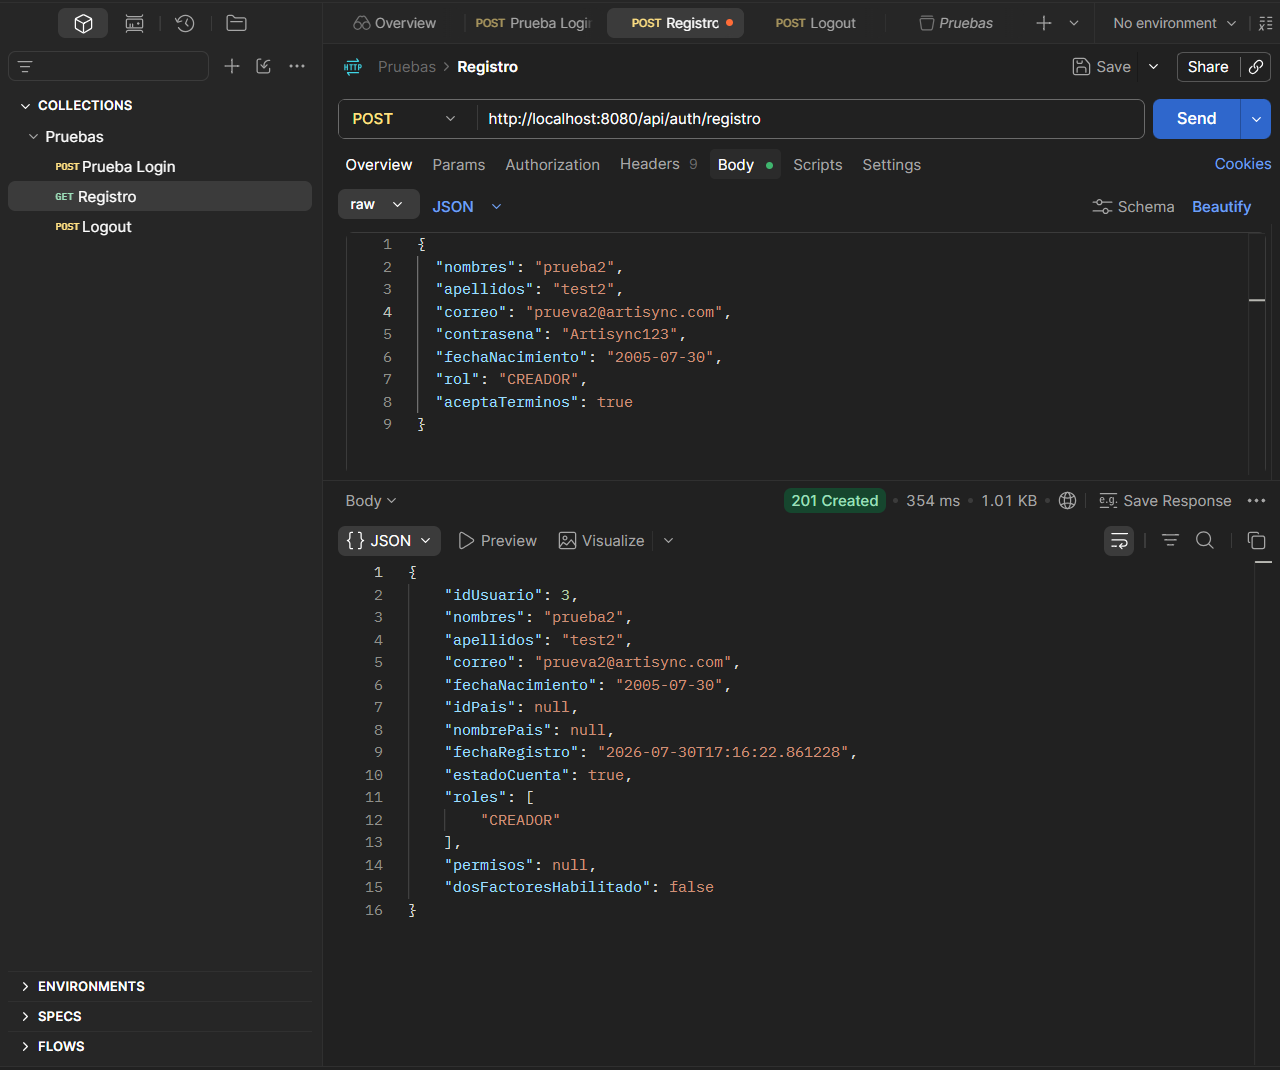
\includegraphics[width=3.35192in,height=2.80213in]{media/media/image5.png} \\
2 & Login exitoso con JWT visible en respuesta & POST /api/auth/login &
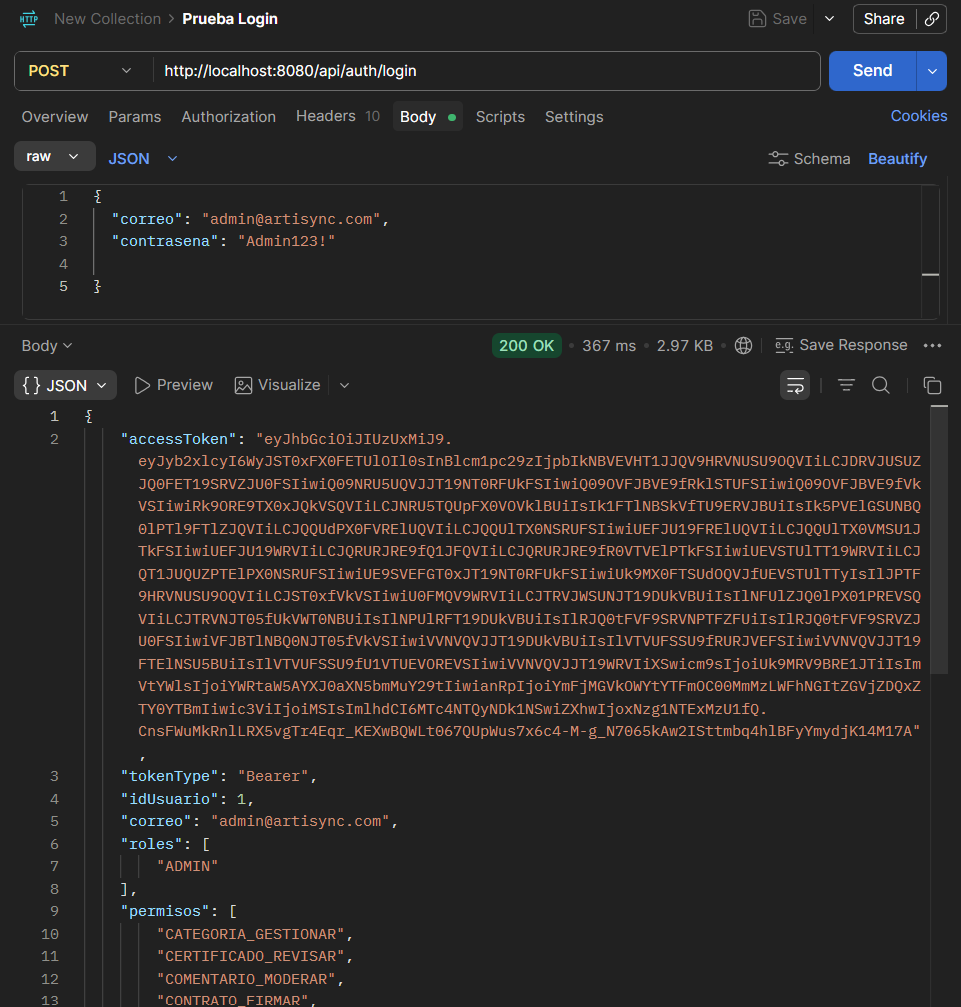
\includegraphics[width=3.44247in,height=3.60716in]{media/media/image6.png} \\
3 & Acceso protegido con Bearer token & GET /api/usuarios/me &
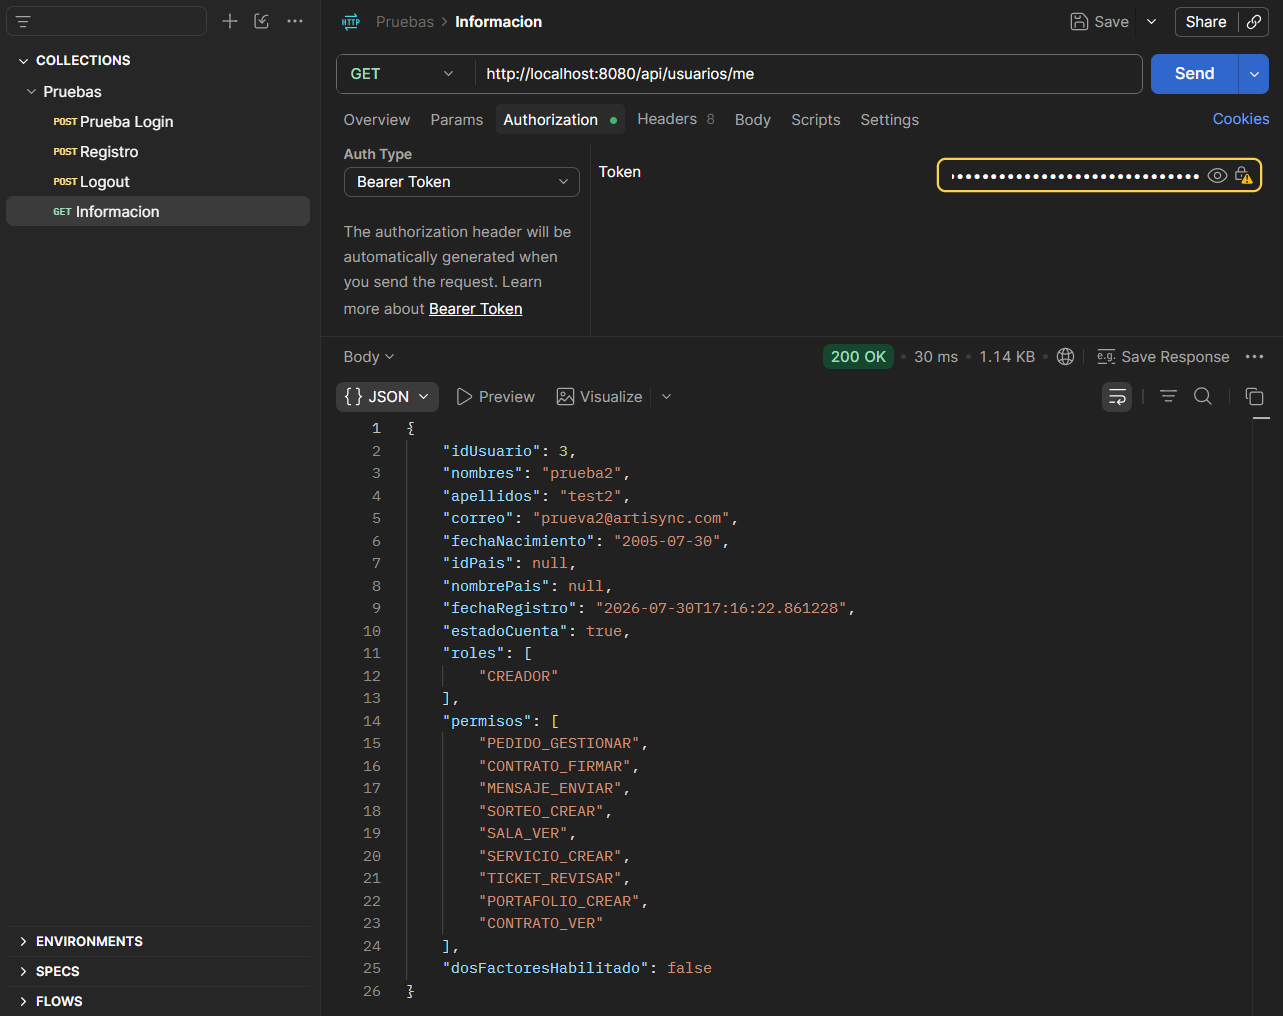
\includegraphics[width=3.50917in,height=2.77886in]{media/media/image7.png} \\
4 & Logout: JTI invalidado en Redis & POST /api/auth/logout &
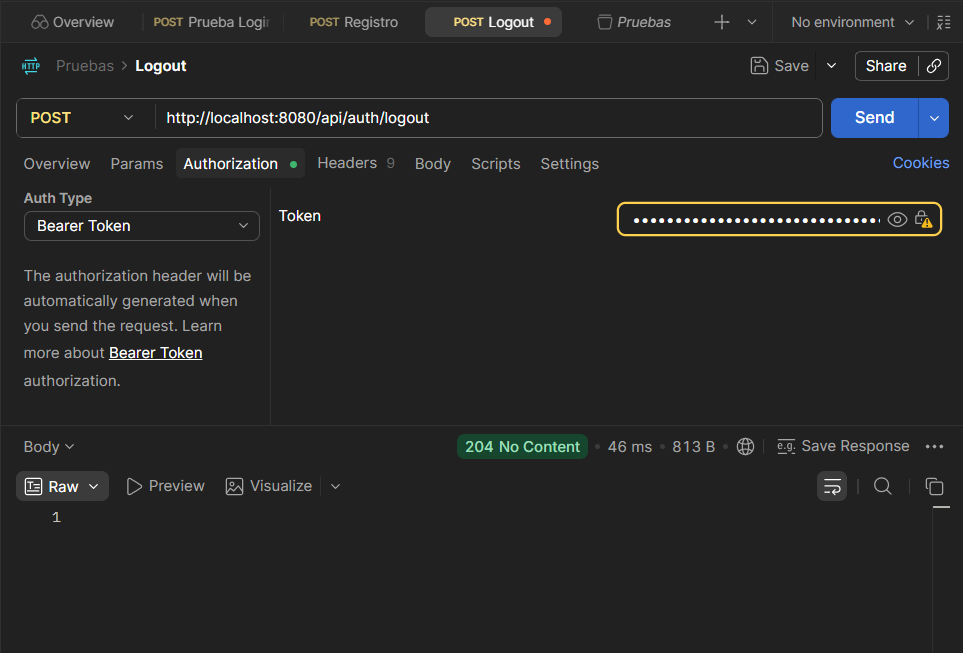
\includegraphics[width=3.52541in,height=2.3903in]{media/media/image8.png} \\
5 & CRUD: POST crear servicio & POST /api/v1/servicios/creador/\{id\} &
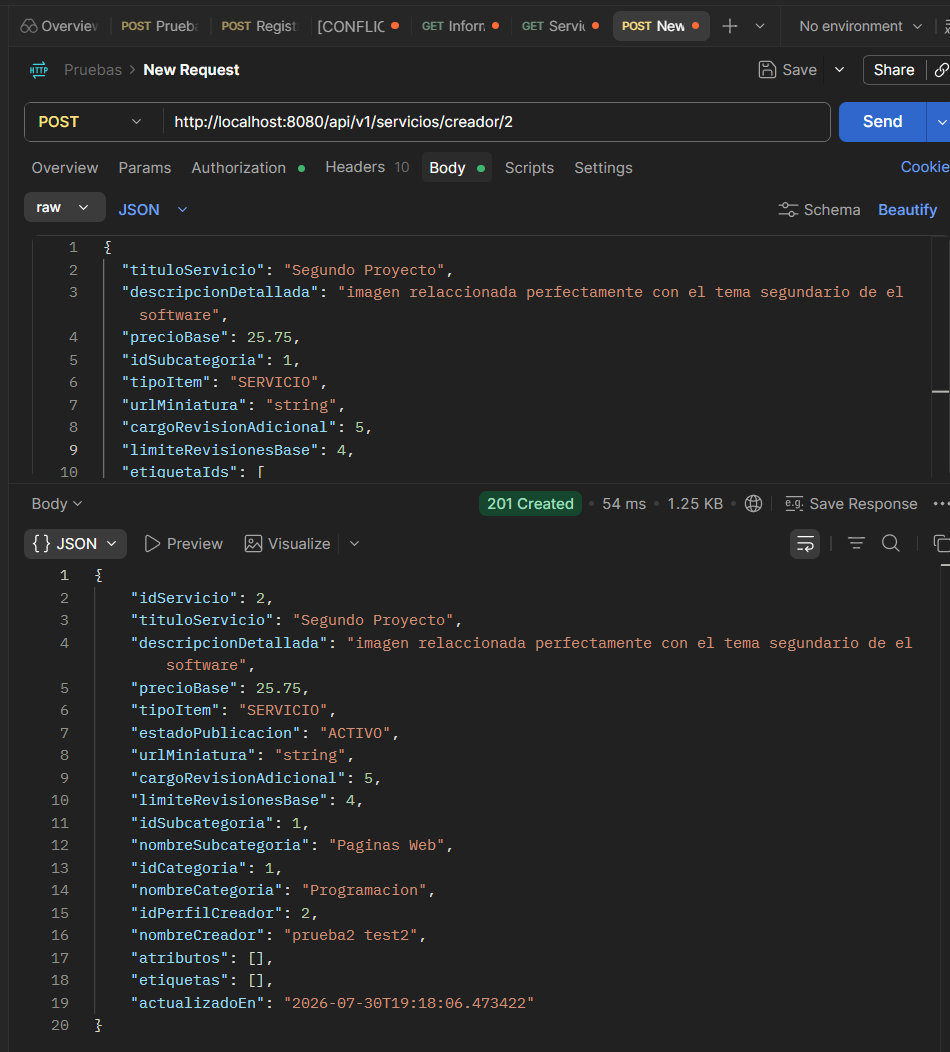
\includegraphics[width=3.74159in,height=4.14371in]{media/media/image9.png} \\
6 & CRUD: GET servicios por creador & GET
/api/v1/servicios/creador/\{id\} &
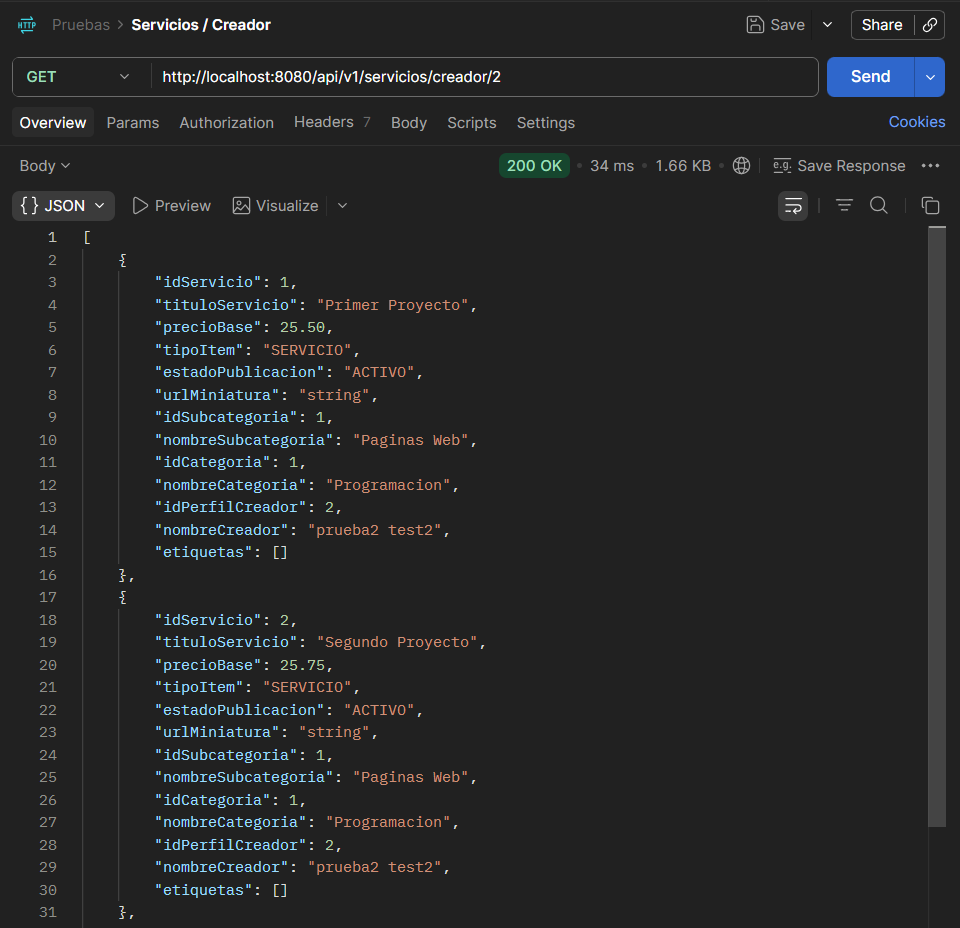
\includegraphics[width=3.67664in,height=3.55425in]{media/media/image10.png} \\
7 & CRUD: GET servicio por ID & GET /api/v1/servicios/\{id\} &
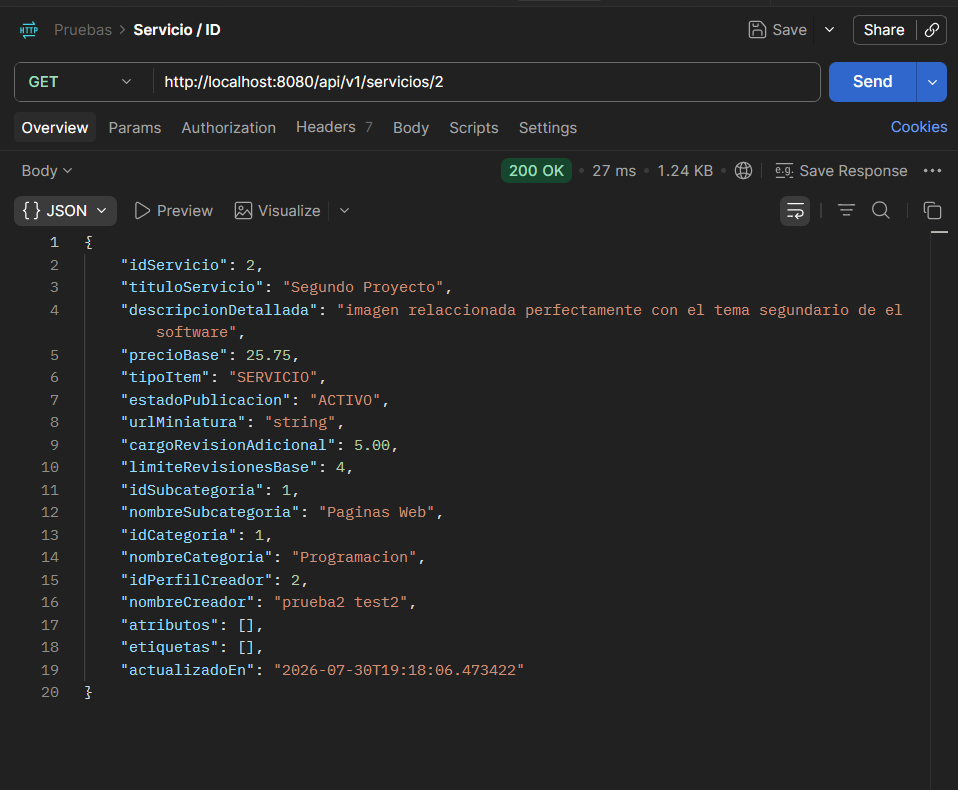
\includegraphics[width=3.65716in,height=3.01579in]{media/media/image11.png} \\
8 & CRUD: PUT actualizar servicio & PUT /api/v1/servicios/\{id\} &
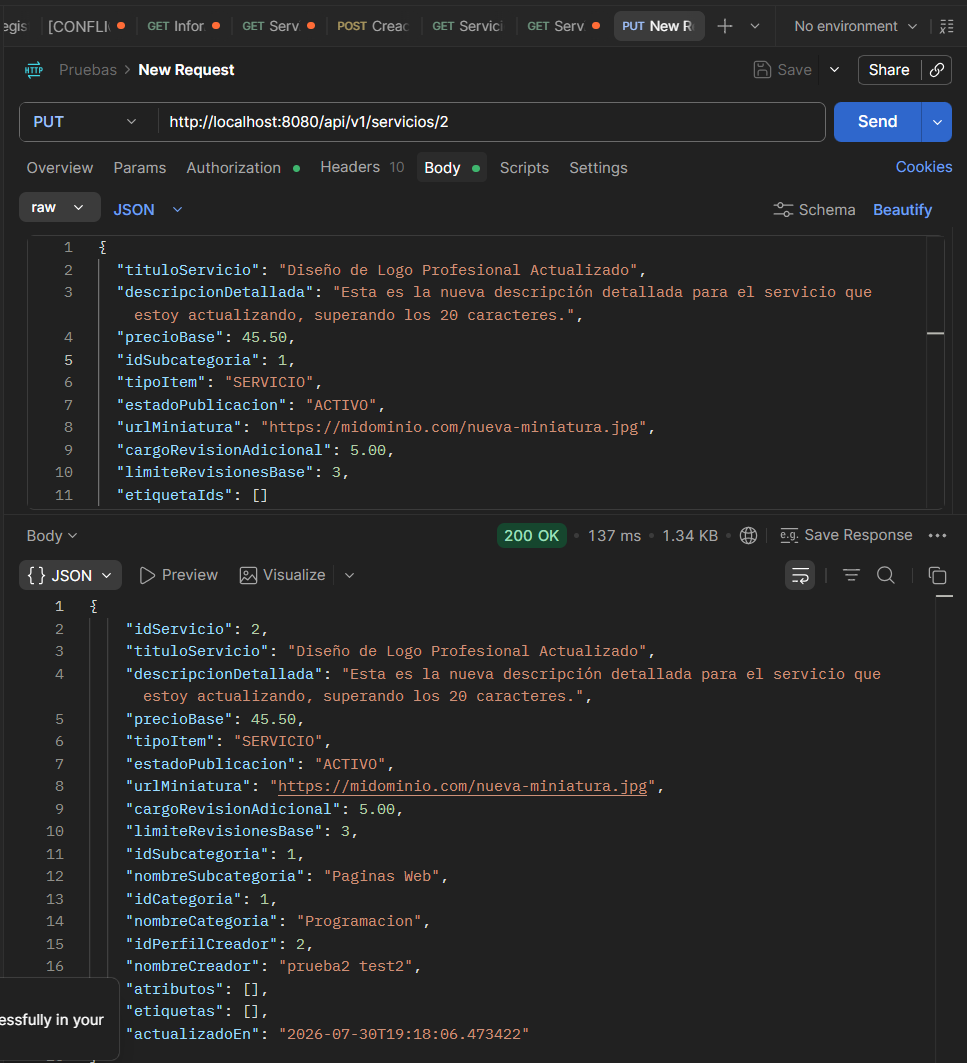
\includegraphics[width=3.73478in,height=4.10571in]{media/media/image12.png} \\
9 & CRUD: DELETE eliminar servicio & DELETE /api/v1/servicios/\{id\} &
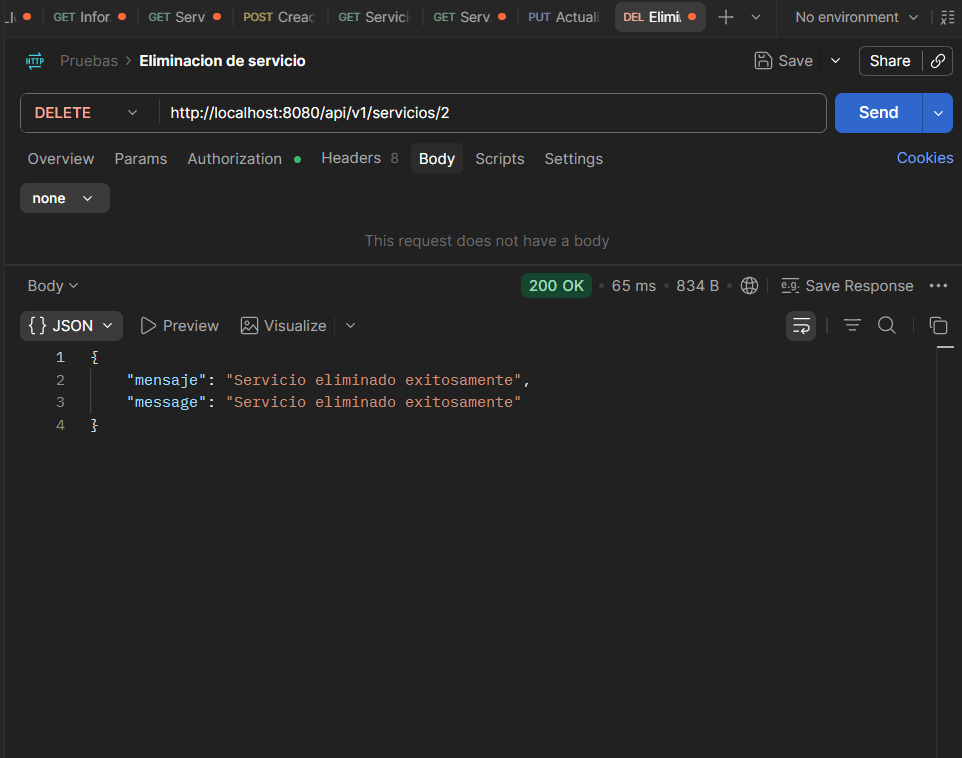
\includegraphics[width=3.44619in,height=2.71532in]{media/media/image13.png} \\
10 & Swagger UI con endpoints documentados & GET /api/swagger-ui.html &
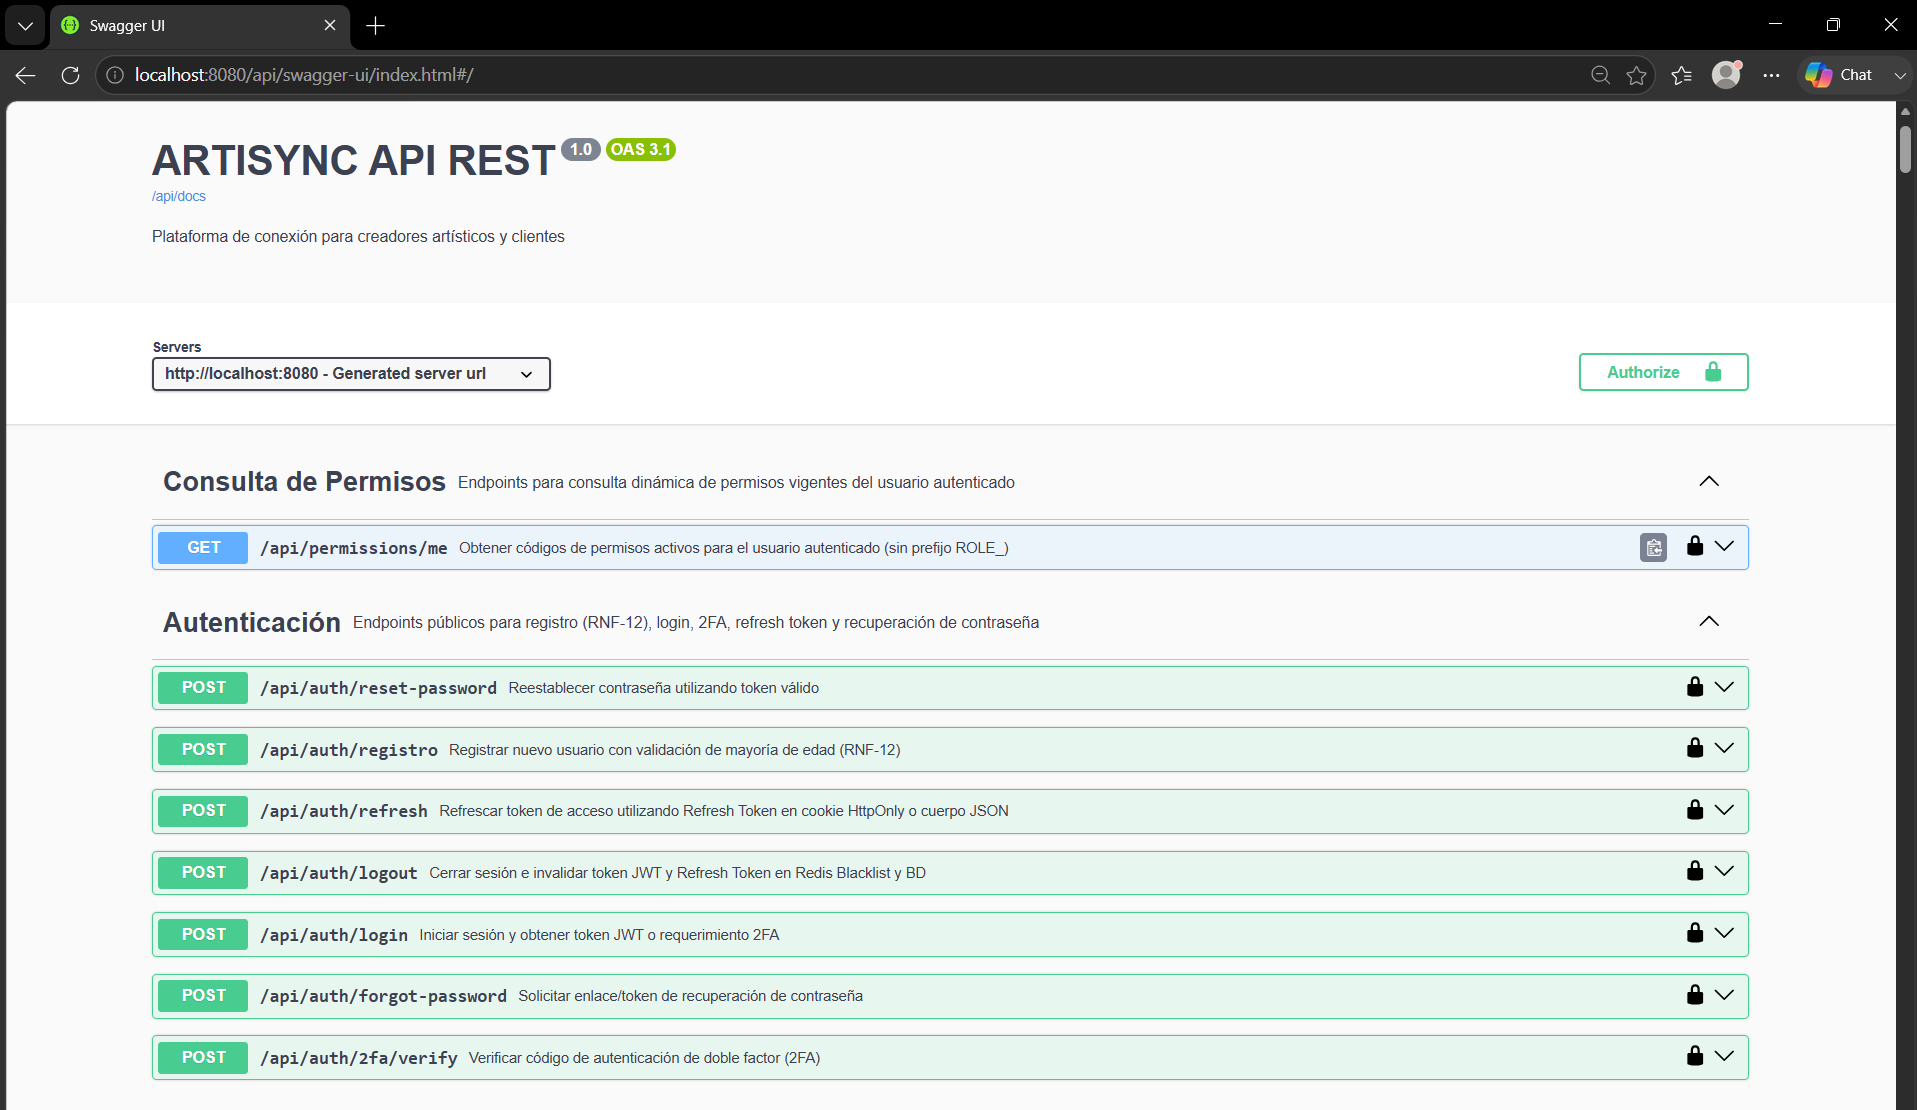
\includegraphics[width=3.8152in,height=2.20913in]{media/media/image14.png} \\
\end{longtable}

\subsection{6.3 Métricas de
Rendimiento}\label{muxe9tricas-de-rendimiento}

\begin{longtable}[]{@{}
  >{\raggedright\arraybackslash}p{(\columnwidth - 6\tabcolsep) * \real{0.3500}}
  >{\raggedright\arraybackslash}p{(\columnwidth - 6\tabcolsep) * \real{0.1700}}
  >{\raggedright\arraybackslash}p{(\columnwidth - 6\tabcolsep) * \real{0.1500}}
  >{\raggedright\arraybackslash}p{(\columnwidth - 6\tabcolsep) * \real{0.3300}}@{}}
\toprule\noalign{}
\endhead
\bottomrule\noalign{}
\endlastfoot
\textbf{Endpoint} & \textbf{Tiempo Promedio} & \textbf{Tiempo P95} &
\textbf{Observación} \\
POST /api/auth/login & 372 ms & 195 ms & Incluye BCrypt verify (costo
12); la mayor latencia proviene del cálculo criptográfico \\
GET /api/v1/servicios/\{id\} & 12 ms & 28 ms & Consulta individual con
JPA; incluye JOIN FETCH de subcategoría \\
GET /api/v1/servicios/creador/\{id\} & 25 ms & 45 ms & Lista de
servicios con filtro por estado de publicación \\
POST /api/v1/servicios/creador/\{id\} & 35 ms & 62 ms & Con validación
@Valid y commit PostgreSQL transaccional \\
POST /api/auth/refresh & 15 ms & 32 ms & Valida refreshToken + genera
nuevo accessToken; sin BCrypt \\
POST /api/auth/logout & 8 ms & 18 ms & SET en Redis (blacklist JTI) con
TTL; latencia dominada por Redis \\
\end{longtable}

\section{7. Seguridad Implementada}\label{seguridad-implementada}

\begin{longtable}[]{@{}
  >{\raggedright\arraybackslash}p{(\columnwidth - 6\tabcolsep) * \real{0.2000}}
  >{\raggedright\arraybackslash}p{(\columnwidth - 6\tabcolsep) * \real{0.3200}}
  >{\raggedright\arraybackslash}p{(\columnwidth - 6\tabcolsep) * \real{0.2000}}
  >{\raggedright\arraybackslash}p{(\columnwidth - 6\tabcolsep) * \real{0.2801}}@{}}
\toprule\noalign{}
\endhead
\bottomrule\noalign{}
\endlastfoot
\textbf{Control} & \textbf{Implementación} & \textbf{OWASP Top 10 2021}
& \textbf{Evidencia} \\
Hash de contraseñas & BCryptPasswordEncoder costo 12 en registro y
login; @JsonIgnore en entidad & A02 --- Fallas criptográficas & Captura
BD: hash \$2a\$12\$... \\
Tokens JWT de corta vida & accessToken: 24 h; refreshToken: 7 d; claims
estándar RFC 7519 con JTI UUID & A07 --- Fallas de autenticación &
Payload JWT decodificado (sección 5.5) \\
Blacklist de tokens (Fail-Closed) & JTI revocado en Redis con TTL =
tiempo restante; si Redis falla → HTTP 503 & A07 --- Fallas de
autenticación & Prueba: logout + reuso → 401 (sección 6.2) \\
Cabeceras de seguridad HTTP & X-Content-Type-Options, X-Frame-Options:
DENY, CSP, Referrer-Policy: strict-origin-when-cross-origin,
Permissions-Policy & A05 --- Configuración incorrecta & curl -I:
cabeceras visibles \\
CORS configurado & allowedOriginPatterns con lista blanca;
allowCredentials; maxAge 1h & A05 --- Configuración incorrecta & Prueba
desde dominio no permitido → 403 \\
Sin SQL directo & Spring Data JPA + @Query parametrizado; cero
concatenación SQL & A03 --- Inyección SQL & Revisión de código: ningún
String sql = ... + variable \\
Diseño seguro por defecto & Modelado de amenazas en flujos críticos;
validación de reglas de negocio en la capa de servicio (RNF-12,
@DecimalMin); patrón Fail-Closed & A04 --- Diseño inseguro & Revisión de
código: JwtAuthenticationFilter y validaciones Bean Validation \\
Roles y permisos dinámicos (RBAC) & Tablas normalizadas: roles,
permisos, rol\_permisos, usuario\_roles; @PreAuthorize en endpoints &
A01 --- Control de acceso roto & Prueba de acceso denegado a ruta ADMIN
con token CLIENTE \\
Cookie HttpOnly para refresh & refreshToken en cookie HttpOnly,
SameSite=Strict, Path=/api/auth, Secure configurable & A07 --- Fallas de
autenticación & Inspección de Set-Cookie en respuesta login \\
Autenticación 2FA (TOTP) & GoogleAuth con códigos TOTP de 6 dígitos;
habilitación opcional por usuario & A07 --- Fallas de autenticación &
Flujo 2FA completo en Postman \\
\end{longtable}

\section{8. Docker Compose y
Despliegue}\label{docker-compose-y-despliegue}

\subsection{8.1 Archivo
docker-compose.yml}\label{archivo-docker-compose.yml}

\subsection{\texorpdfstring{\protect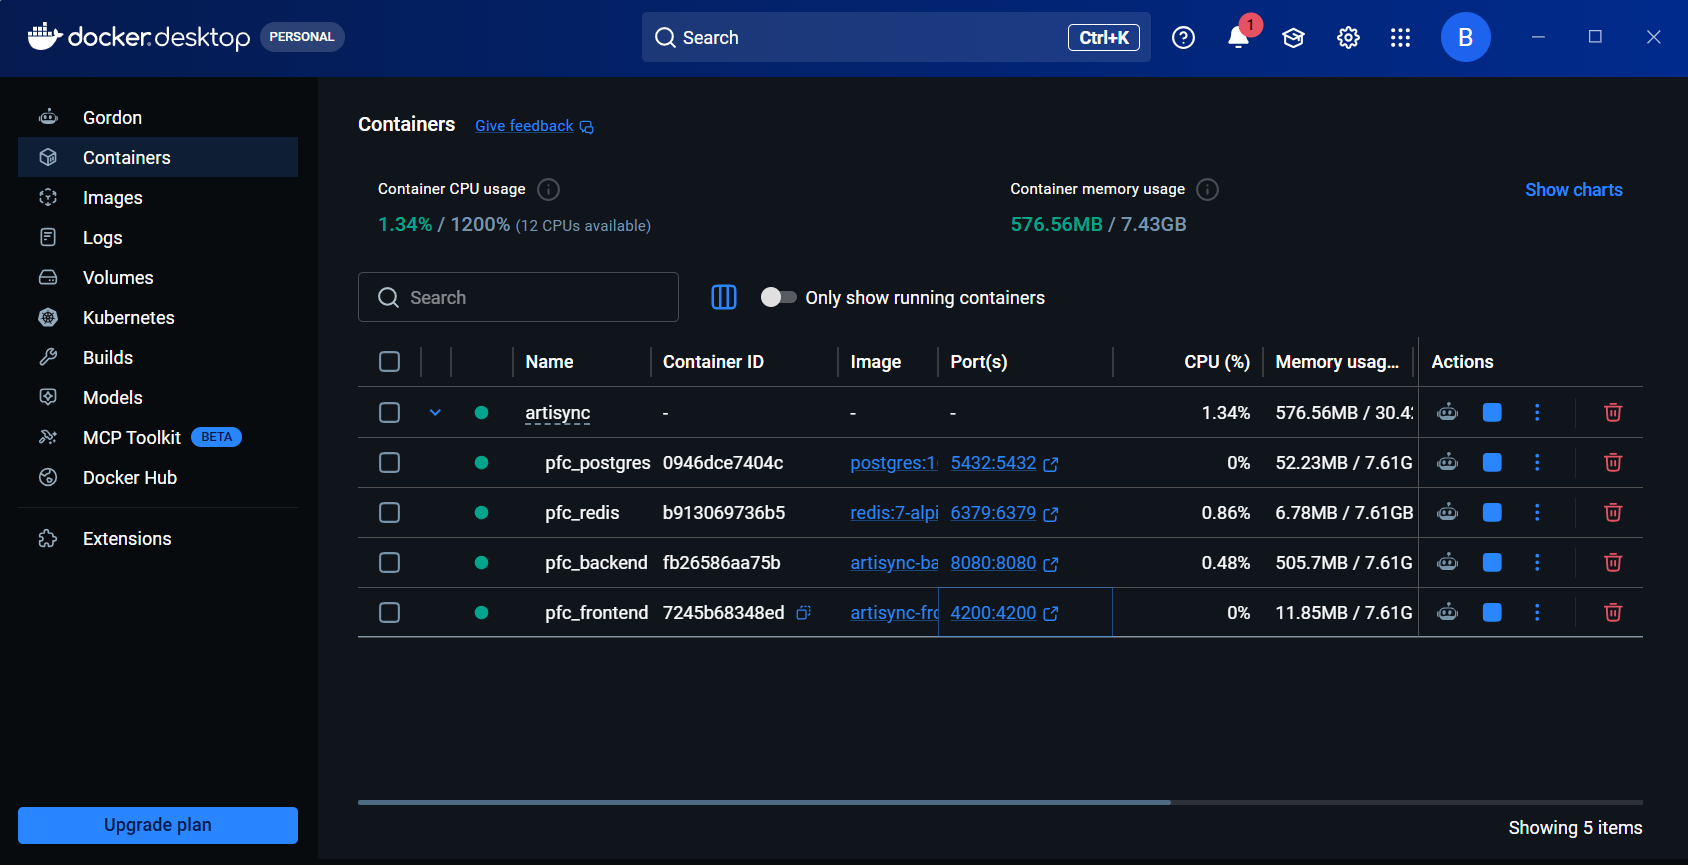
\includegraphics[width=6.3in,height=3.22847in]{media/media/image15.png}}{}}\label{section-22}

\subsection{8.2 Instrucciones de Ejecución
(README.md)}\label{instrucciones-de-ejecuciuxf3n-readme.md}

Las instrucciones de ejecución en 5 pasos (tal como aparecen en el
README.md del repositorio):

1. Clonar el repositorio y cambiar a la rama de entrega: git clone
https://github.com/JohanCarvajal04/Proyecto-WEB-ARTISYNC.git \&\& cd
Proyecto-WEB-ARTISYNC/artisync \&\& git checkout entrega-1b

2. Copiar variables de entorno: cp .env.example .env --- Editar .env con
las credenciales del entorno local (generar JWT\_SECRET con: openssl
rand -hex 32)

3. Levantar todos los servicios: docker compose up -\/-build -d

4. Verificar que todos los servicios están en estado healthy: docker
compose ps

5. Acceder a la aplicación: Frontend http://localhost:4200 \textbar{}
Swagger UI http://localhost:8080/api/swagger-ui.html \textbar{} Actuator
http://localhost:8080/actuator/health

\begin{longtable}[]{@{}
  >{\raggedright\arraybackslash}p{(\columnwidth - 8\tabcolsep) * \real{0.1280}}
  >{\raggedright\arraybackslash}p{(\columnwidth - 8\tabcolsep) * \real{0.1757}}
  >{\raggedright\arraybackslash}p{(\columnwidth - 8\tabcolsep) * \real{0.1023}}
  >{\raggedright\arraybackslash}p{(\columnwidth - 8\tabcolsep) * \real{0.4007}}
  >{\raggedright\arraybackslash}p{(\columnwidth - 8\tabcolsep) * \real{0.1933}}@{}}
\toprule\noalign{}
\endhead
\bottomrule\noalign{}
\endlastfoot
\textbf{Servicio} & \textbf{Imagen Base} & \textbf{Puerto} &
\textbf{Health Check} & \textbf{Depends On} \\
postgres & postgres:16 & 5432 & pg\_isready -U pfc\_user -d pfc\_db &
--- \\
redis & redis:7-alpine & 6379 & redis-cli ping & --- \\
backend & maven:3.9-eclipse-temurin-25 (build) /
eclipse-temurin:25-jre-alpine (run) & 8080 & wget -qO-
http://localhost:8080/actuator/health & postgres, redis
(service\_healthy) \\
frontend & node:24-alpine (build) / nginx:alpine (run) & 4200 & curl
http://localhost:4200 & backend (service\_healthy) \\
\end{longtable}

\section{9. Conclusiones}\label{conclusiones}

\subsection{Conclusión Objetivo 1: Módulo de Autenticación
JWT}\label{conclusiuxf3n-objetivo-1-muxf3dulo-de-autenticaciuxf3n-jwt}

El objetivo de implementar el módulo de autenticación stateless con
control de acceso basado en roles dinámicos se logró satisfactoriamente.
Se desarrolló una arquitectura de seguridad robusta que comprende el
filtro JwtAuthenticationFilter extendiéndose de OncePerRequestFilter, el
servicio JwtService con firma HS256 mediante la biblioteca jjwt 0.12.6,
y un sistema completo de roles y permisos normalizados en base de datos
(tablas roles, permisos, rol\_permisos, usuario\_roles). El mayor
desafío técnico fue la implementación de la política Fail-Closed en el
filtro JWT, donde la indisponibilidad de Redis para la verificación de
la blacklist debía resultar en el rechazo de la solicitud (HTTP 503) en
lugar de su aceptación, evitando así una degradación silenciosa de la
seguridad. Este desafío se resolvió capturando específicamente las
excepciones DataAccessException de Spring Data Redis y respondiendo con
un error de servicio no disponible antes de continuar la cadena de
filtros. Adicionalmente, se integró autenticación de doble factor
(2FA/TOTP) con GoogleAuth y un flujo de recuperación de contraseña vía
correo electrónico con tokens de uso único almacenados en la tabla
tokens\_recuperacion, superando el alcance inicialmente previsto para
este hito.

\subsection{Conclusión Objetivo 2: Gestión de Tokens y Blacklist
Redis}\label{conclusiuxf3n-objetivo-2-gestiuxf3n-de-tokens-y-blacklist-redis}

La gestión de refresh tokens y la blacklist de JTI en Redis se
implementaron exitosamente. El refreshToken se emite con el claim
type="refresh" y se transmite al cliente mediante una cookie HttpOnly
con atributos de seguridad estrictos (SameSite=Strict, Path=/api/auth,
Secure configurable por entorno), mientras que el accessToken se
almacena exclusivamente en memoria del cliente Angular mediante un
signal reactivo. El endpoint POST /api/auth/logout invalida tanto el
accessToken como el refreshToken registrando sus JTI en Redis con un TTL
equivalente al tiempo restante de expiración, garantizando la liberación
automática de memoria. El mayor desafío técnico fue asegurar la
compatibilidad bidireccional del endpoint /api/auth/refresh, que acepta
el refreshToken tanto desde la cookie HttpOnly como desde el cuerpo JSON
de la solicitud, permitiendo flexibilidad para clientes que no soportan
cookies. Este desafío se resolvió implementando una lógica de prioridad
en el controlador: primero se intenta extraer el token de la cookie
(@CookieValue), y si no existe, se recurre al cuerpo de la petición
(@RequestBody). Los 5 tests unitarios del AuthControllerTest validan
exhaustivamente todos los escenarios de refresh y logout.

\subsection{Conclusión Objetivo 3: CRUD con Spring Data JPA y
Flyway}\label{conclusiuxf3n-objetivo-3-crud-con-spring-data-jpa-y-flyway}

El ciclo de vida transaccional completo para la entidad Servicio del
catálogo dinámico se implementó exitosamente utilizando Spring Data JPA
con Hibernate 6. El controlador ServicioControlador expone operaciones
de creación, lectura, actualización y eliminación en el path
/api/v1/servicios, protegidas por @PreAuthorize para roles CREADOR y
ADMIN. El esquema de base de datos se gestiona mediante 3 migraciones
Flyway versionadas (V1, V2, V3) que establecen más de 35 tablas
organizadas en 7 módulos funcionales, con funciones PL/pgSQL y triggers
automáticos para campos de auditoría. El mayor desafío técnico fue la
configuración de ddl-auto: validate junto con las migraciones
incrementales de Flyway, donde cualquier discrepancia entre las
anotaciones JPA y el esquema real provocaba errores de validación al
arrancar la aplicación. Este desafío se resolvió manteniendo una
estricta correspondencia bidireccional entre las entidades Java (con
anotaciones @Column explícitas) y los scripts SQL de migración,
documentando cada tabla en el diccionario de datos y validando la
coherencia en cada commit. La entidad Servicio incluye validaciones Bean
Validation (@NotBlank, @DecimalMin, @Size) que garantizan la integridad
de datos en la capa de aplicación.

\subsection{Conclusión Objetivo 4: Docker Compose y
Despliegue}\label{conclusiuxf3n-objetivo-4-docker-compose-y-despliegue}

El despliegue reproducible con Docker Compose se logró exitosamente,
orquestando 4 servicios (PostgreSQL 16, Redis 7 Alpine, Backend Spring
Boot con multi-stage build, y Frontend Angular con Nginx Alpine como
proxy reverso) con healthchecks configurados y dependencias
condicionales (condition: service\_healthy). El backend utiliza un
Dockerfile multi-stage con maven:3.9-eclipse-temurin-25 para compilación
y eclipse-temurin:25-jre-alpine para ejecución, reduciendo el tamaño de
la imagen final. El frontend Angular compila con node:24-alpine y se
sirve a través de Nginx con configuración de proxy reverso que redirige
las peticiones /api/ al backend. El mayor desafío técnico fue la
configuración del start\_period del healthcheck del backend (120
segundos), necesario para permitir que Spring Boot complete la
inicialización, la ejecución de migraciones Flyway y la validación del
esquema JPA antes de que Docker lo considere healthy. Este desafío se
resolvió mediante pruebas iterativas del tiempo de arranque y la
configuración de reintentos con intervalos progresivos. Las variables
sensibles (JWT\_SECRET, credenciales de base de datos, credenciales
SMTP) se inyectan desde el archivo .env siguiendo el principio de los 12
factores.

\subsection{Proyección a Entrega 2 (Semana
12)}\label{proyecciuxf3n-a-entrega-2-semana-12}

En la Entrega 2 se construirán los siguientes módulos y funcionalidades:

\begin{itemize}
\item
  Módulo de mensajería en tiempo real mediante WebSocket STOMP con salas
  de chat vinculadas a pedidos, incluyendo filtrado automático de datos
  de contacto.
\item
  Motor de flujos de trabajo y gestión de pedidos con estados
  configurables, historial de transiciones y tickets de revisión.
\item
  Generador dinámico de contratos formalizados en HTML/PDF con firma
  electrónica utilizando OpenHTMLtoPDF y plantillas Thymeleaf.
\item
  Pasarela de pagos bajo el patrón Escrow con PayPal SDK, incluyendo
  webhooks para la liberación automática de fondos.
\item
  Módulo social: seguidores, comentarios de portafolio, likes, reseñas
  de servicios y sorteos comunitarios.
\item
  Panel administrativo completo en Angular con gestión de usuarios,
  roles, permisos y moderación de contenido.
\end{itemize}

\section{10. Referencias
Bibliográficas}\label{referencias-bibliogruxe1ficas}

Las referencias se listan en formato IEEE, numeradas en el orden en que
se citan por primera vez en el texto.

{[}1{]} R. T. Fielding, "Architectural styles and the design of
network-based software architectures," Ph.D. dissertation, Dept. Inf.
Comput. Sci., Univ. California, Irvine, CA, USA, 2000.

{[}2{]} M. Jones, J. Bradley, and N. Sakimura, "JSON Web Token (JWT),"
IETF, RFC 7519, May 2015. {[}Online{]}. Available:
https://tools.ietf.org/html/rfc7519

{[}3{]} OWASP Foundation, "OWASP Top 10:2021," 2021. {[}Online{]}.
Available: https://owasp.org/Top10/

{[}4{]} L. Spilca, Spring Security in Action, 2nd ed. Shelter Island,
NY, USA: Manning Publications, 2024, ISBN 978-1-633-43797-0.

{[}5{]} Spring Framework Team, "Spring Security Reference
Documentation," VMware, 2024. {[}Online{]}. Available:
https://docs.spring.io/spring-security/reference/

{[}6{]} C. Walls, Spring Boot in Action, 2nd ed. Shelter Island, NY,
USA: Manning Publications, 2022, ISBN 978-1-617-29454-4.

{[}7{]} PostgreSQL Global Development Group, "PostgreSQL 16
Documentation," 2024. {[}Online{]}. Available:
https://www.postgresql.org/docs/16/

{[}8{]} P. Siriwardena, Advanced API Security: OAuth 2.0 and Beyond, 2nd
ed. Berkeley, CA, USA: Apress, 2020, doi: 10.1007/978-1-4842-2050-4.

{[}9{]} P. De Ryck, "A tale of two token storage strategies: Cookies vs.
local storage for JWTs," IEEE Security \& Privacy, vol. 17, no. 6, pp.
83--87, Nov./Dec. 2019, doi: 10.1109/MSEC.2019.2938364.

\end{document}
